%% Reykjavik University Presentation Template by Joseph T. Foley < foley AT ru DOT is >
\documentclass[aspectratio=169]{rubeamer}
%% Add option "icelandic" to switch sections and labels
%% Add one of these options to change the aspect ratio:
%% 1610 149 54 43 32 which is 16:10 14:9 etc.

%% If you have customizations and packages you use a lot, put them in custom-beamer.sty
%% It will be automatically loaded if it exists
%% I have loaded this with packages and macros I find useful


%%----------- Citations ---------------------------
%% I highly advise using JabRef to manage your .bib files.
%% It can catch a lot of errors early and helps you fill things in.
%% In particular, you probably want to set it to fix line endings to NL only in the preferences.

%%%% Now pick a citation style
%%IEEE citations (just numbers)
%\usepackage[backend=biber, bibencoding=utf8, style=ieee]{biblatex}

%% APA style (author, year) -- need all of these lines
%\usepackage[backend=biber, bibencoding=utf8, style=apa]{biblatex}
%\usepackage[american]{babel}
%\DeclareLanguageMapping{american}{american-apa}  % after biblatex and babel

%% Alphabetic (abbrv-year), more compact
\usepackage[backend=biber, bibencoding=utf8, style=alphabetic]{biblatex}

%\usepackage{multicol}
%\usepackage{multirow}
%\usepackage{array}

%% Put your reference library files here. Don't forget to put the .bib
%% extension. If you have multiple people with their own libraries (or
%% are using the Zotero plugin) it is a good idea to have multiple
%% files separated according to some agreement.  This is the divisions the author uses:

\addbibresource{references.bib}%references specific to this paper
\addbibresource{references-ad.bib}%reference related to Axiomatic Design
\addbibresource{references-foley.bib}%references that the author has participated on.  Helpful for writing a CV.
\addbibresource{references-collections.bib}%Due to BibTeX/Biber processing, multi-author books and proceedings must go last if they are used as crossref.


%% ------------------ Graphics ----------------------------%%
\graphicspath{{graphics/}{Graphics/}}
%% This is a list of folders to search for graphics files to include in that order.
%% Each path should be in a {}.  
%% Make sure that the upper/lowercase of the letters matches the folder or
%% you may have weird problems with partners using other operating systems.

\usepackage{datetime}
\usepackage{hyperref}
\usepackage{textcomp}

\newdateformat{monthyeardate}{\monthname[\THEMONTH] \THEYEAR}

%% -----------------Titles and Footers ---------------------%%
%% The abbreviated information goes in the [], the full information in {}
\title[PhD Thesis Proposal]{Real Time, Onboard-only Landing Site Evaluation for Autonomous Drones}
\subtitle[demo]{PhD Thesis Proposal}
\author[Springer]{Joshua Springer}
\institute[RU]{Reykjavík University}
\date[2022]{\monthyeardate\today}%Set this to when you will present

\newcommand{\nologo}{\setbeamertemplate{logo}{}}
\newcommand{\yeslogo}{\logo{
\includegraphics[width=1.5cm]{ru_logo_transparent}}}

\yeslogo

\newif\ifpause
\pausetrue
%\pausefalse
\newcommand{\mypause}{\ifpause \pause \fi}

\titlegraphic{
\includegraphics[width=2CM]{ru_logo_transparent}}

\AtBeginSection[]{
  \begin{frame}
  \vfill
  \centering
  \begin{beamercolorbox}[sep=8pt,center,shadow=true,rounded=true]{title}
    \usebeamerfont{title}\insertsectionhead\par%
  \end{beamercolorbox}
  \vfill
  \end{frame}
}

\begin{document}

\setbeamercovered{invisible}

%----------- titlepage ----------------------------------------------%
\begin{frame}[plain]%plain option gets rid of the footer and the per-page logo
  \titlepage
%  \begin{textblock}{10}(12,4)
%    
\includegraphics[width=0.3\textwidth]{ru-logo}
%  \end{textblock}

\end{frame}

\begin{frame}
  \frametitle{Presentation Structure}
  \begin{enumerate}
    \item Introduction
      \begin{itemize}
        \item Problem description and motivation
        \item State of the Art
      \end{itemize}
    \item Completed/ongoing projects
      \begin{itemize}
        \item Initial proof of concept attempt
          \begin{itemize}
            \item Continuation of master thesis (tested in simulation)
          \end{itemize}
        \item Fiducial marker modifications
        \item Proof of concept
      \end{itemize}
    \item Research Plan
      \begin{itemize}
        \item Methods
        \item Challenges and risk analysis
      \end{itemize}
  \end{enumerate}
\end{frame}

%----------- slides ----------------------------------------------%
\section{Introduction}

\begin{frame}
  \frametitle{Problem Description and Motivation}
  \begin{columns}
    \column{0.6\textwidth}
    \begin{itemize}
      \item Much of basic drone flight has been \textbf{automated}.
      \mypause
      \begin{itemize}
        \item Takeoff
        \item Waypoint-to-waypoint-flight
        \item Track/orbit objects,\\take pictures, etc.
      \end{itemize}
      \mypause
      \item Landing is still largely \textbf{manual}.
      \mypause
      \begin{itemize}
        \item No continuous, autonomous mission cycles
        \item Primitive, semi-autonomous methods are common (still require human operator)
        \item Hand-catching is common
      \end{itemize}
    \end{itemize}
    \column{0.4\textwidth}
    \centering
    \mypause
    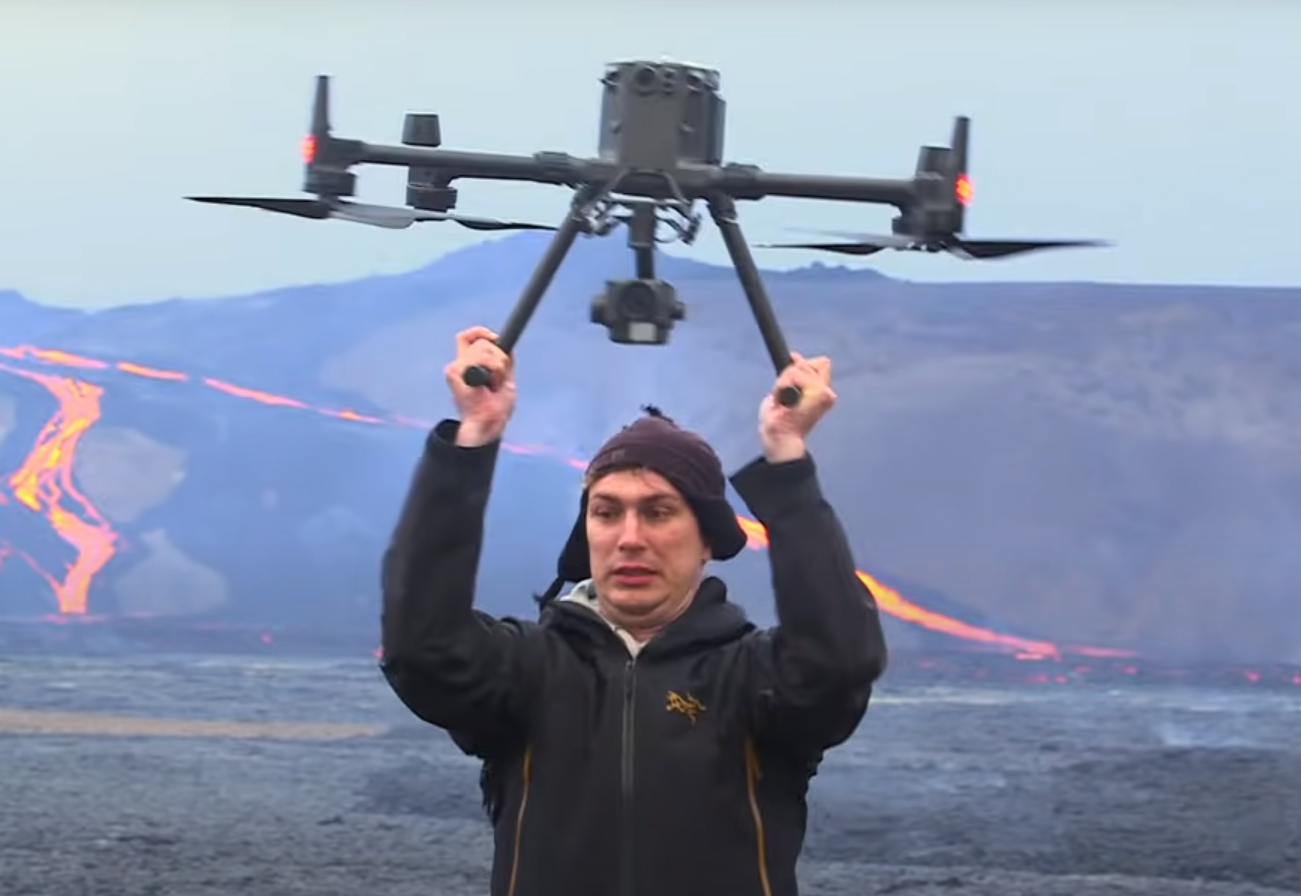
\includegraphics[width=\textwidth]{human_assisted_landing}\\
    ``Human-assisted landing''
  \end{columns}
\end{frame}

\begin{frame}
  \frametitle{Research Questions}
  \begin{itemize}
    \mypause
    \item How can a drone autonomously land?
    \mypause
    \item What data do autonomous drone landing methods need?
    \mypause
    \item How can those methods execute in real time onboard a drone?
  \end{itemize}
\end{frame}

\begin{frame}
  \frametitle{State of the Art}
  \begin{itemize}
    \item GPS-based landing
    \mypause
    \begin{itemize}
      \item RTK
    \end{itemize}
    \mypause
    \item Known landing locations:
    \begin{itemize}
      \item Visual matching
      \mypause
      \item Visual markers
      \mypause
      \item IR beacons
    \end{itemize}
    \mypause
    \item Terrain analysis
    \begin{itemize}
      \item Optical flow\mypause~(requires motion)
      \mypause
      \item RGBD, LIDAR\mypause~(slow, offload processing)
    \end{itemize}
%    \mypause
%    \item Other methods
  \end{itemize}

\end{frame}

\section{Completed and Ongoing Projects}

\begin{frame}
  \frametitle{Test Hexacopters}
  \begin{columns}
    \column{0.5\textwidth}
    \begin{itemize}
      \item Two Tarot 680 hexacopters
      \item For real-world proof of concept of master thesis simulations.
    \end{itemize}
    \column{0.5\textwidth}
    \centering
    \onslide
    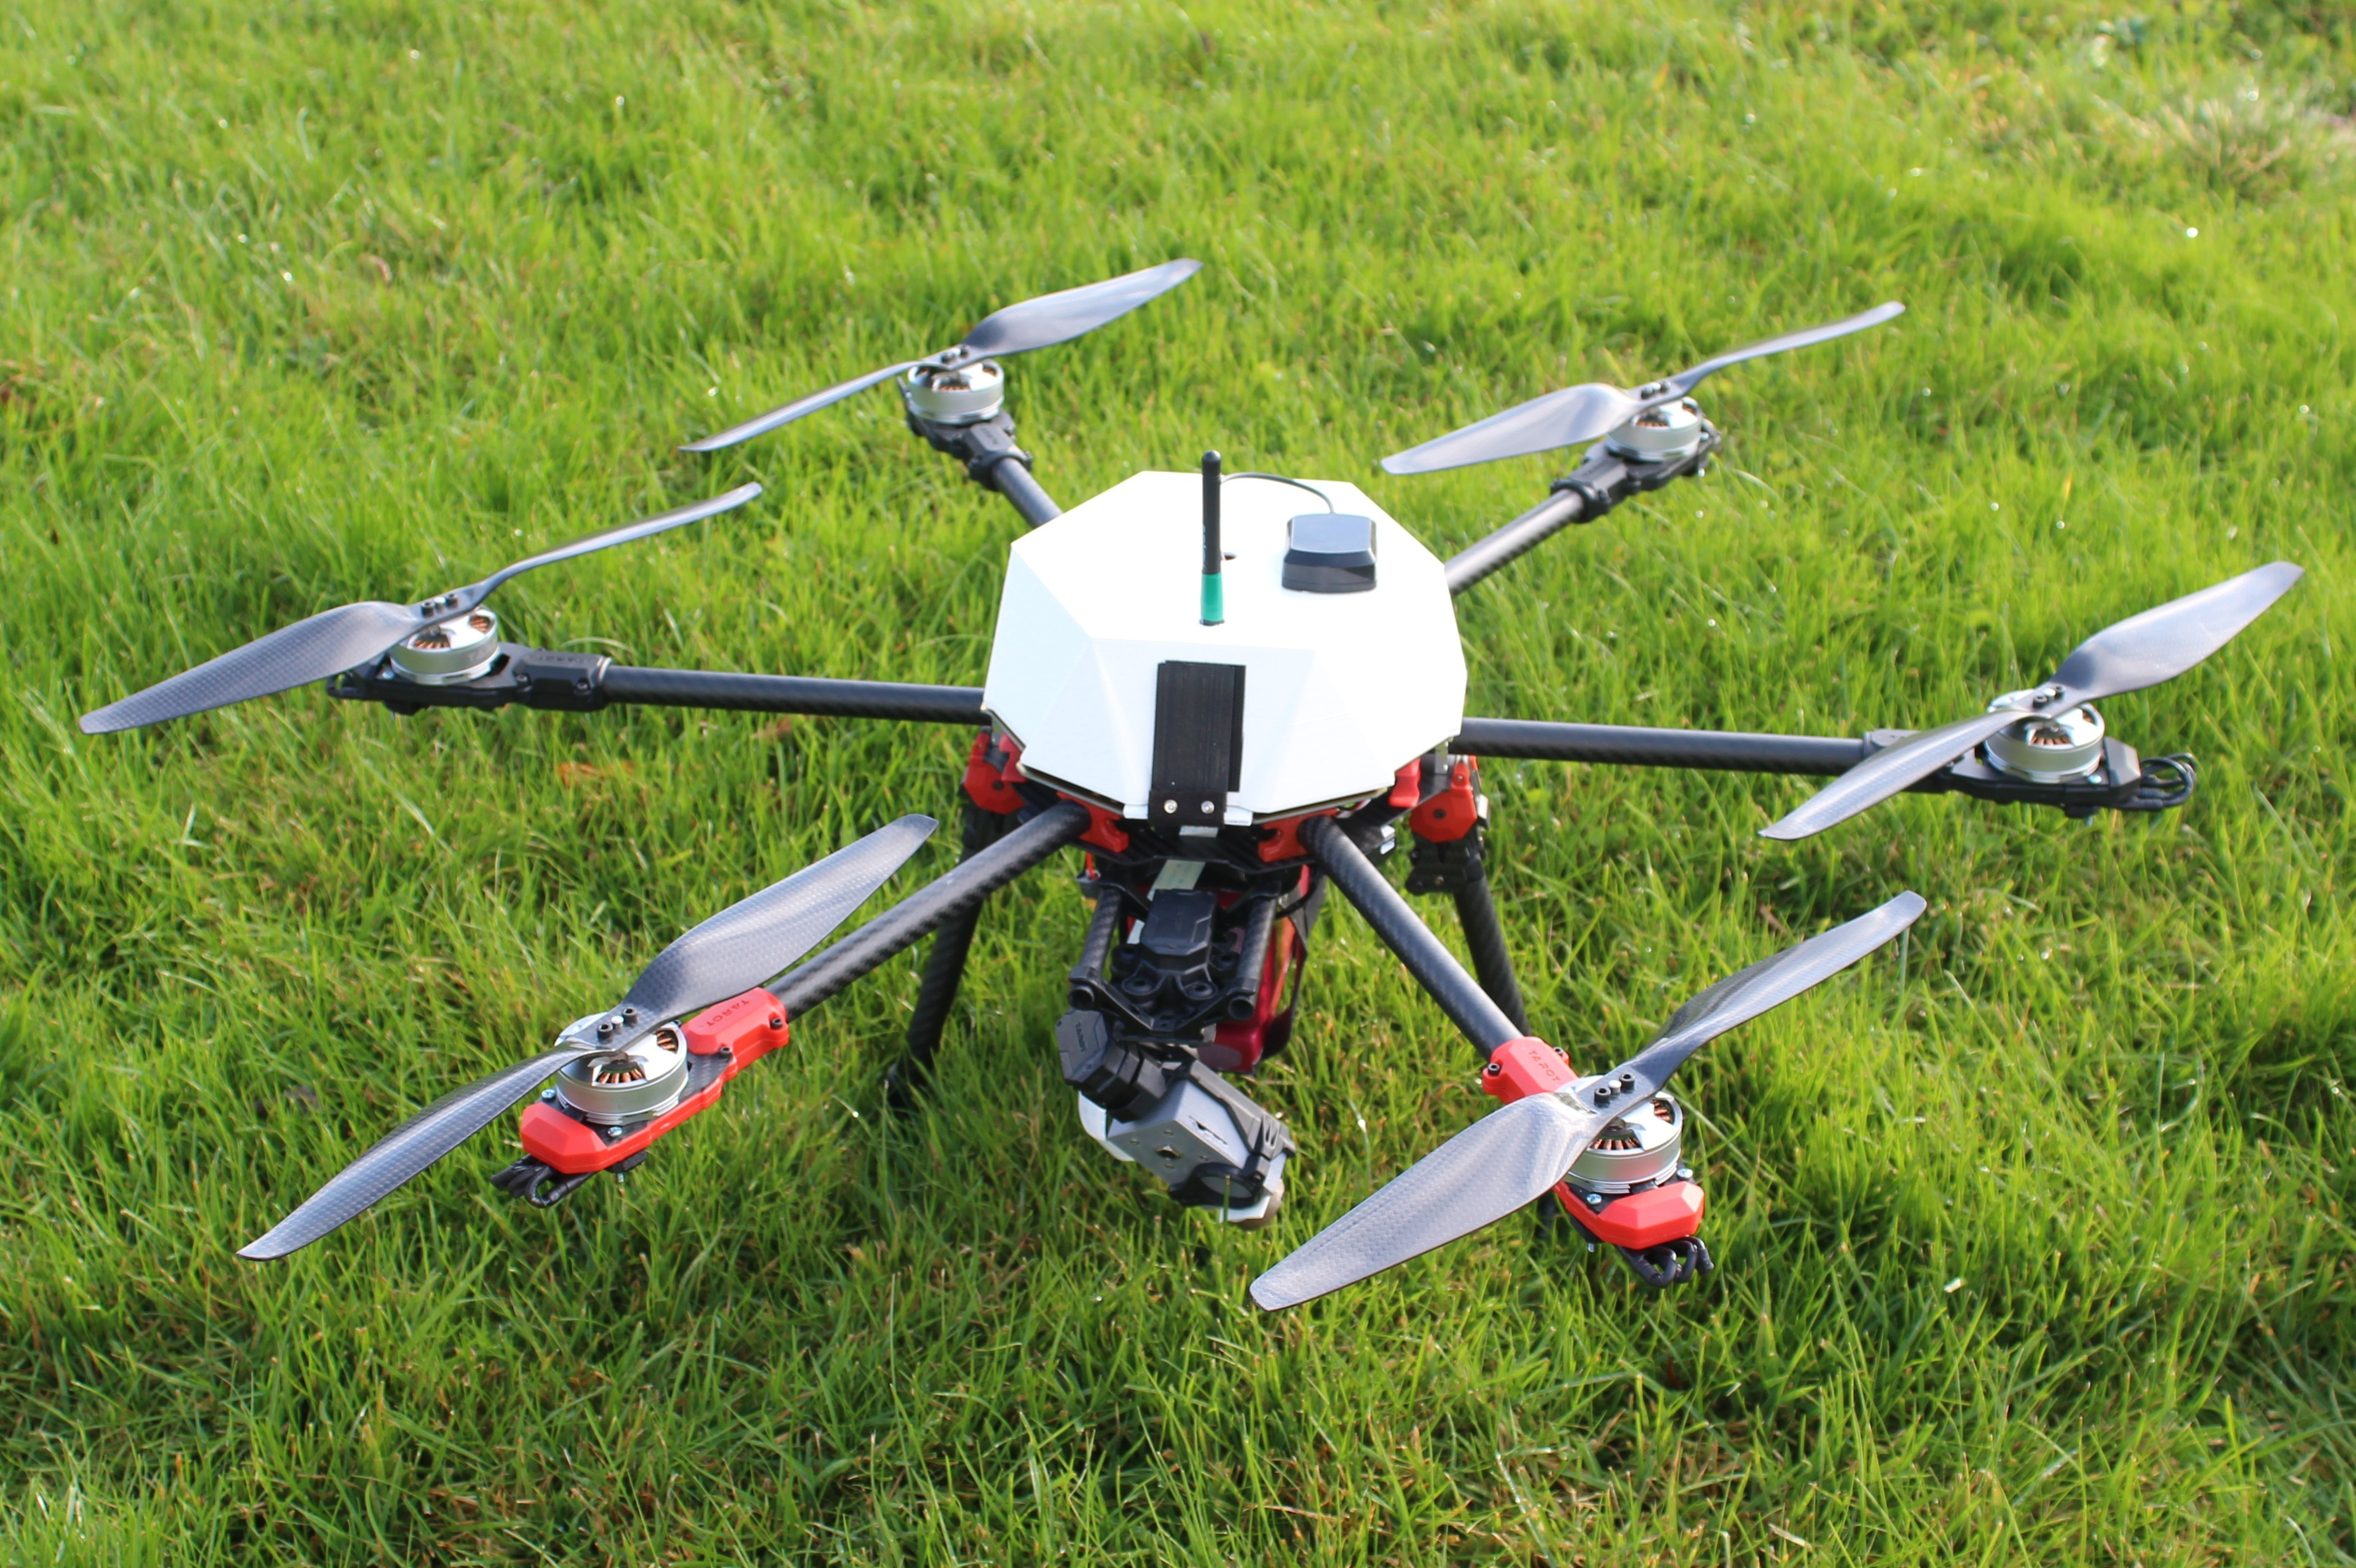
\includegraphics[width=0.75\textwidth]{coral_drone}\\
    \mypause
    
\includegraphics[width=0.35\textwidth, angle=-90]{original_landing_pad}
  \end{columns}
\end{frame}

\begin{frame}
  \frametitle{Test Hexacopter Components}
  \begin{columns}
    \column{0.5\textwidth}
    \begin{itemize}
      \item Navio2 + RPi 3 autopilot combo
      \mypause
      \item Companion boards (for heavy onboard processing):
      \begin{itemize}
        \mypause
        \item Google Coral (embedded TPU)
        \mypause
        \item Jetson Nano (embedded GPU)
      \end{itemize}
      \mypause
      \item Gimbaled camera modules
      \mypause
      \item 433 MHz telemetry
      \mypause
      \item 2.4 GHz R/C control
      \mypause
      \item Tested Autopilot Softwares
      \begin{itemize}
        \item ArduPilot
        \mypause
        \item PX4 (not technically supported)
      \end{itemize}
    \end{itemize}
    \column{0.5\textwidth}
    \centering
    \onslide
    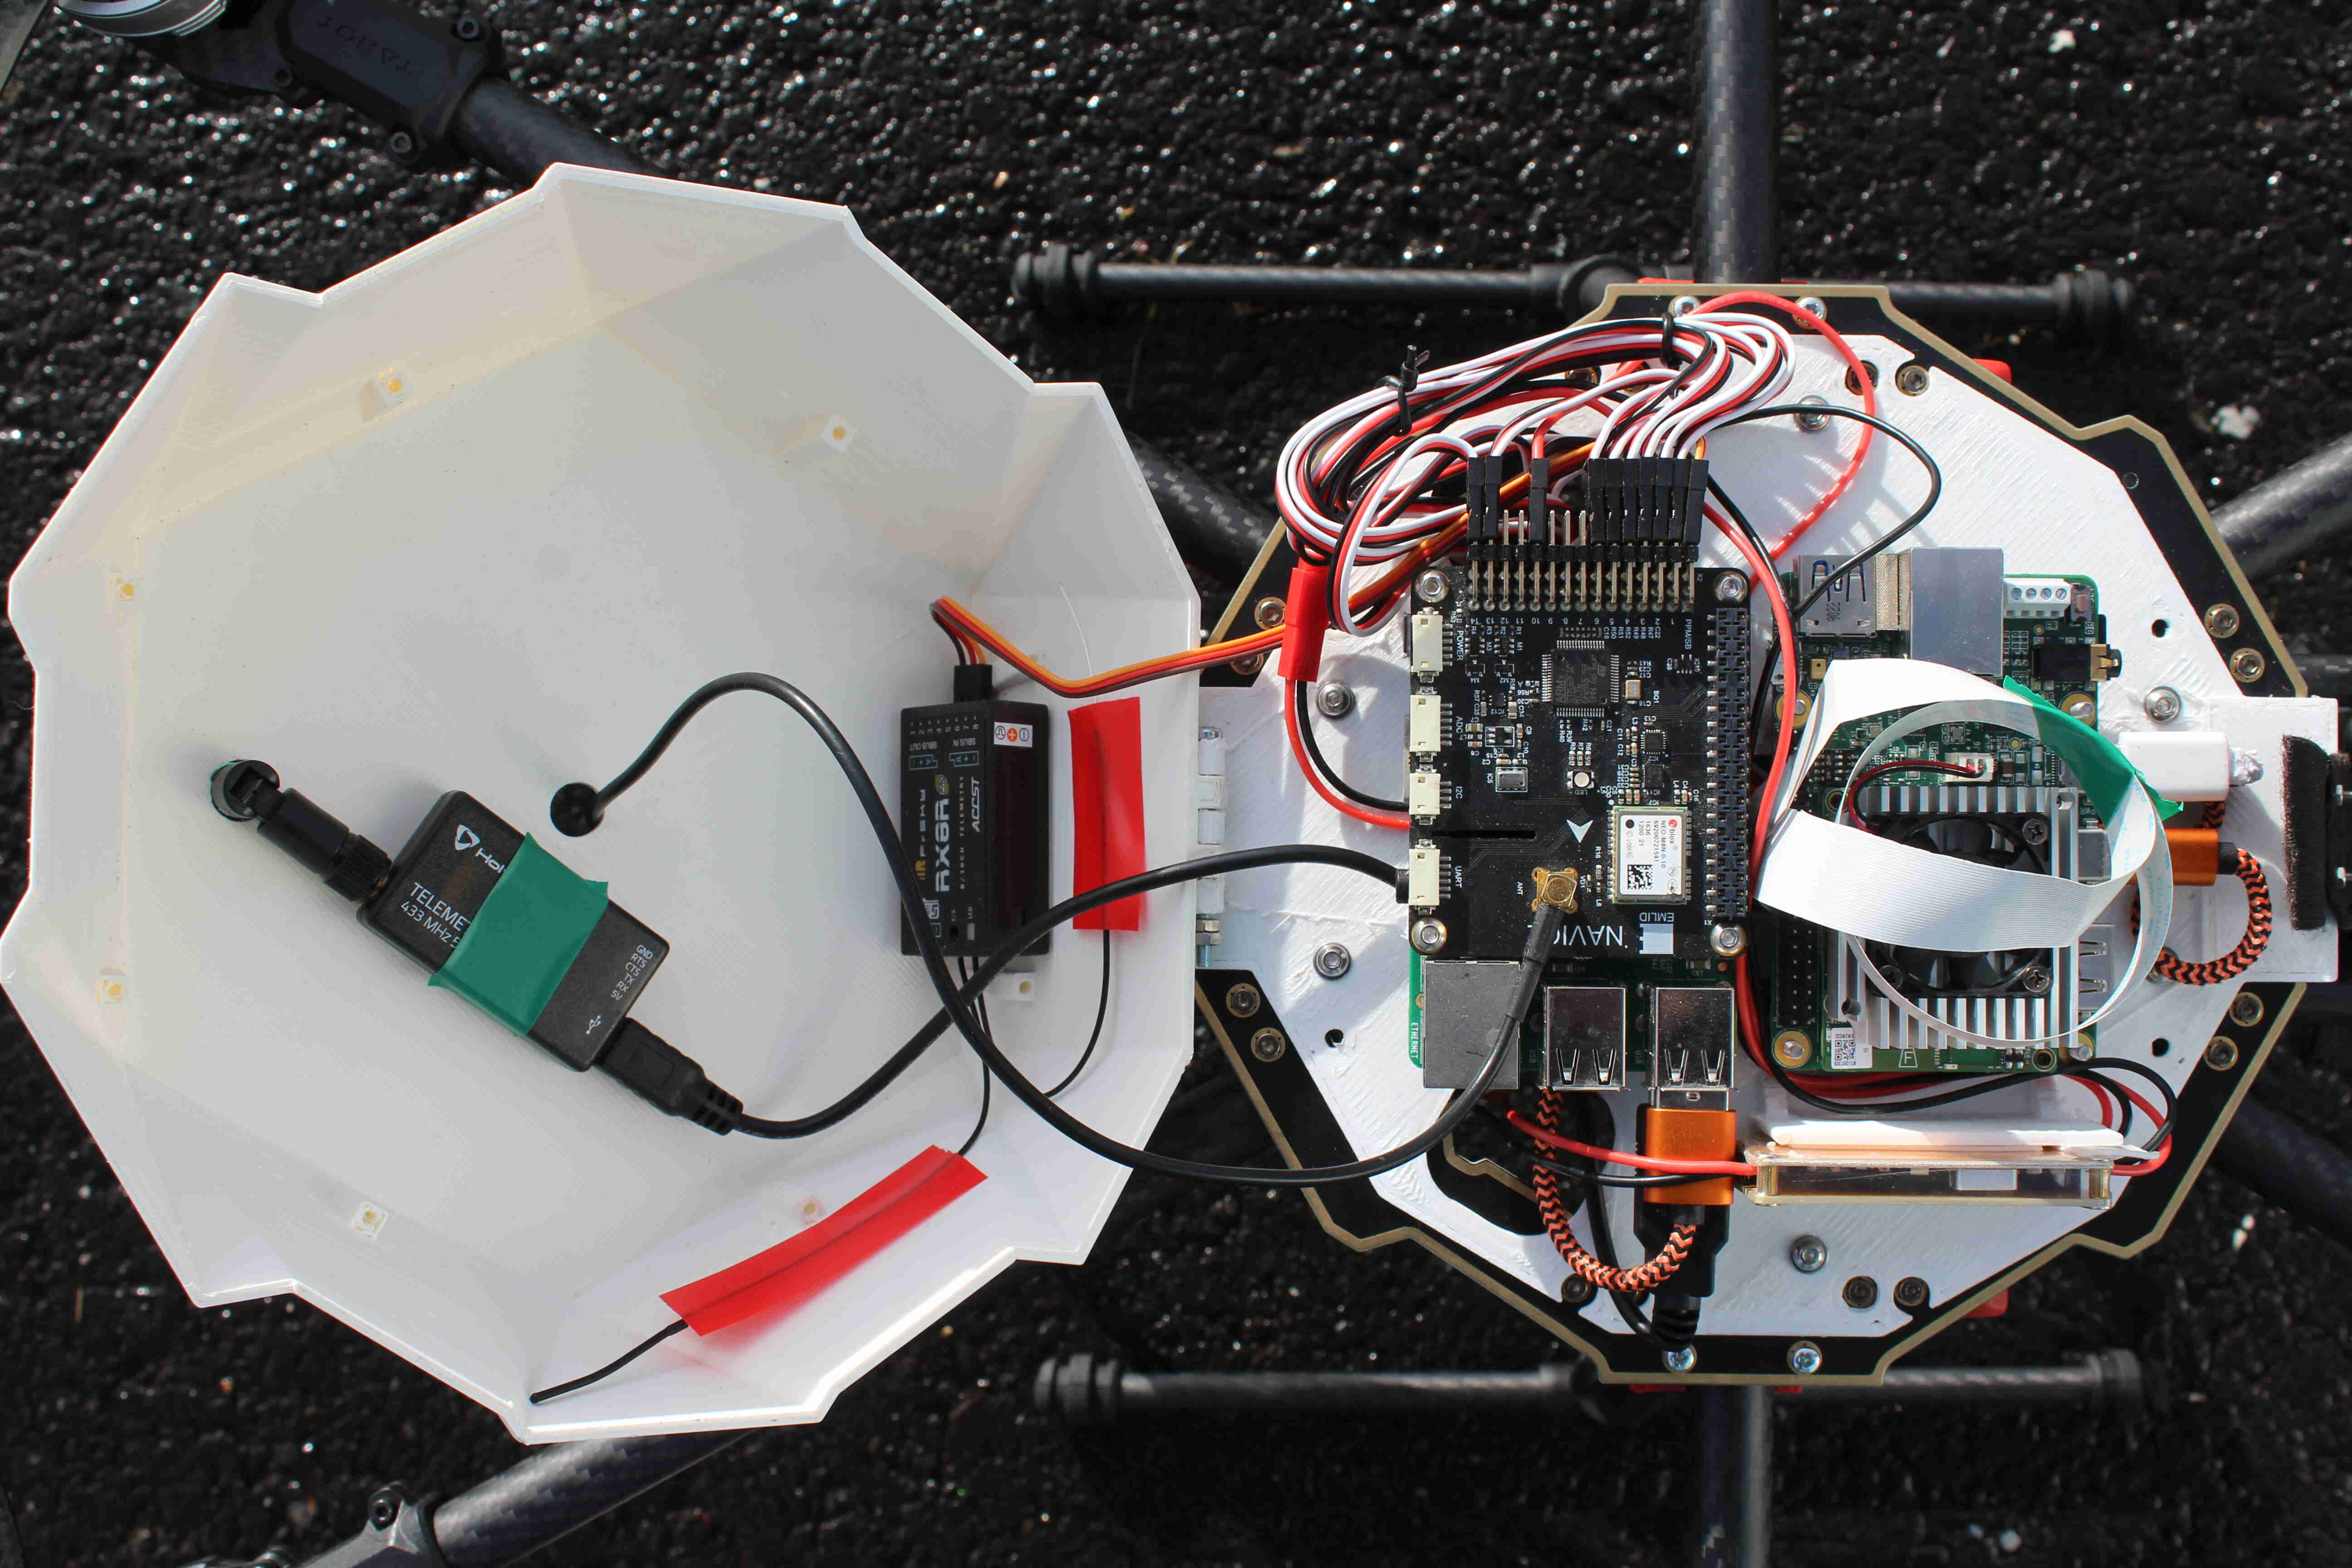
\includegraphics[width=0.6\textwidth]{coral_electronics}\\
    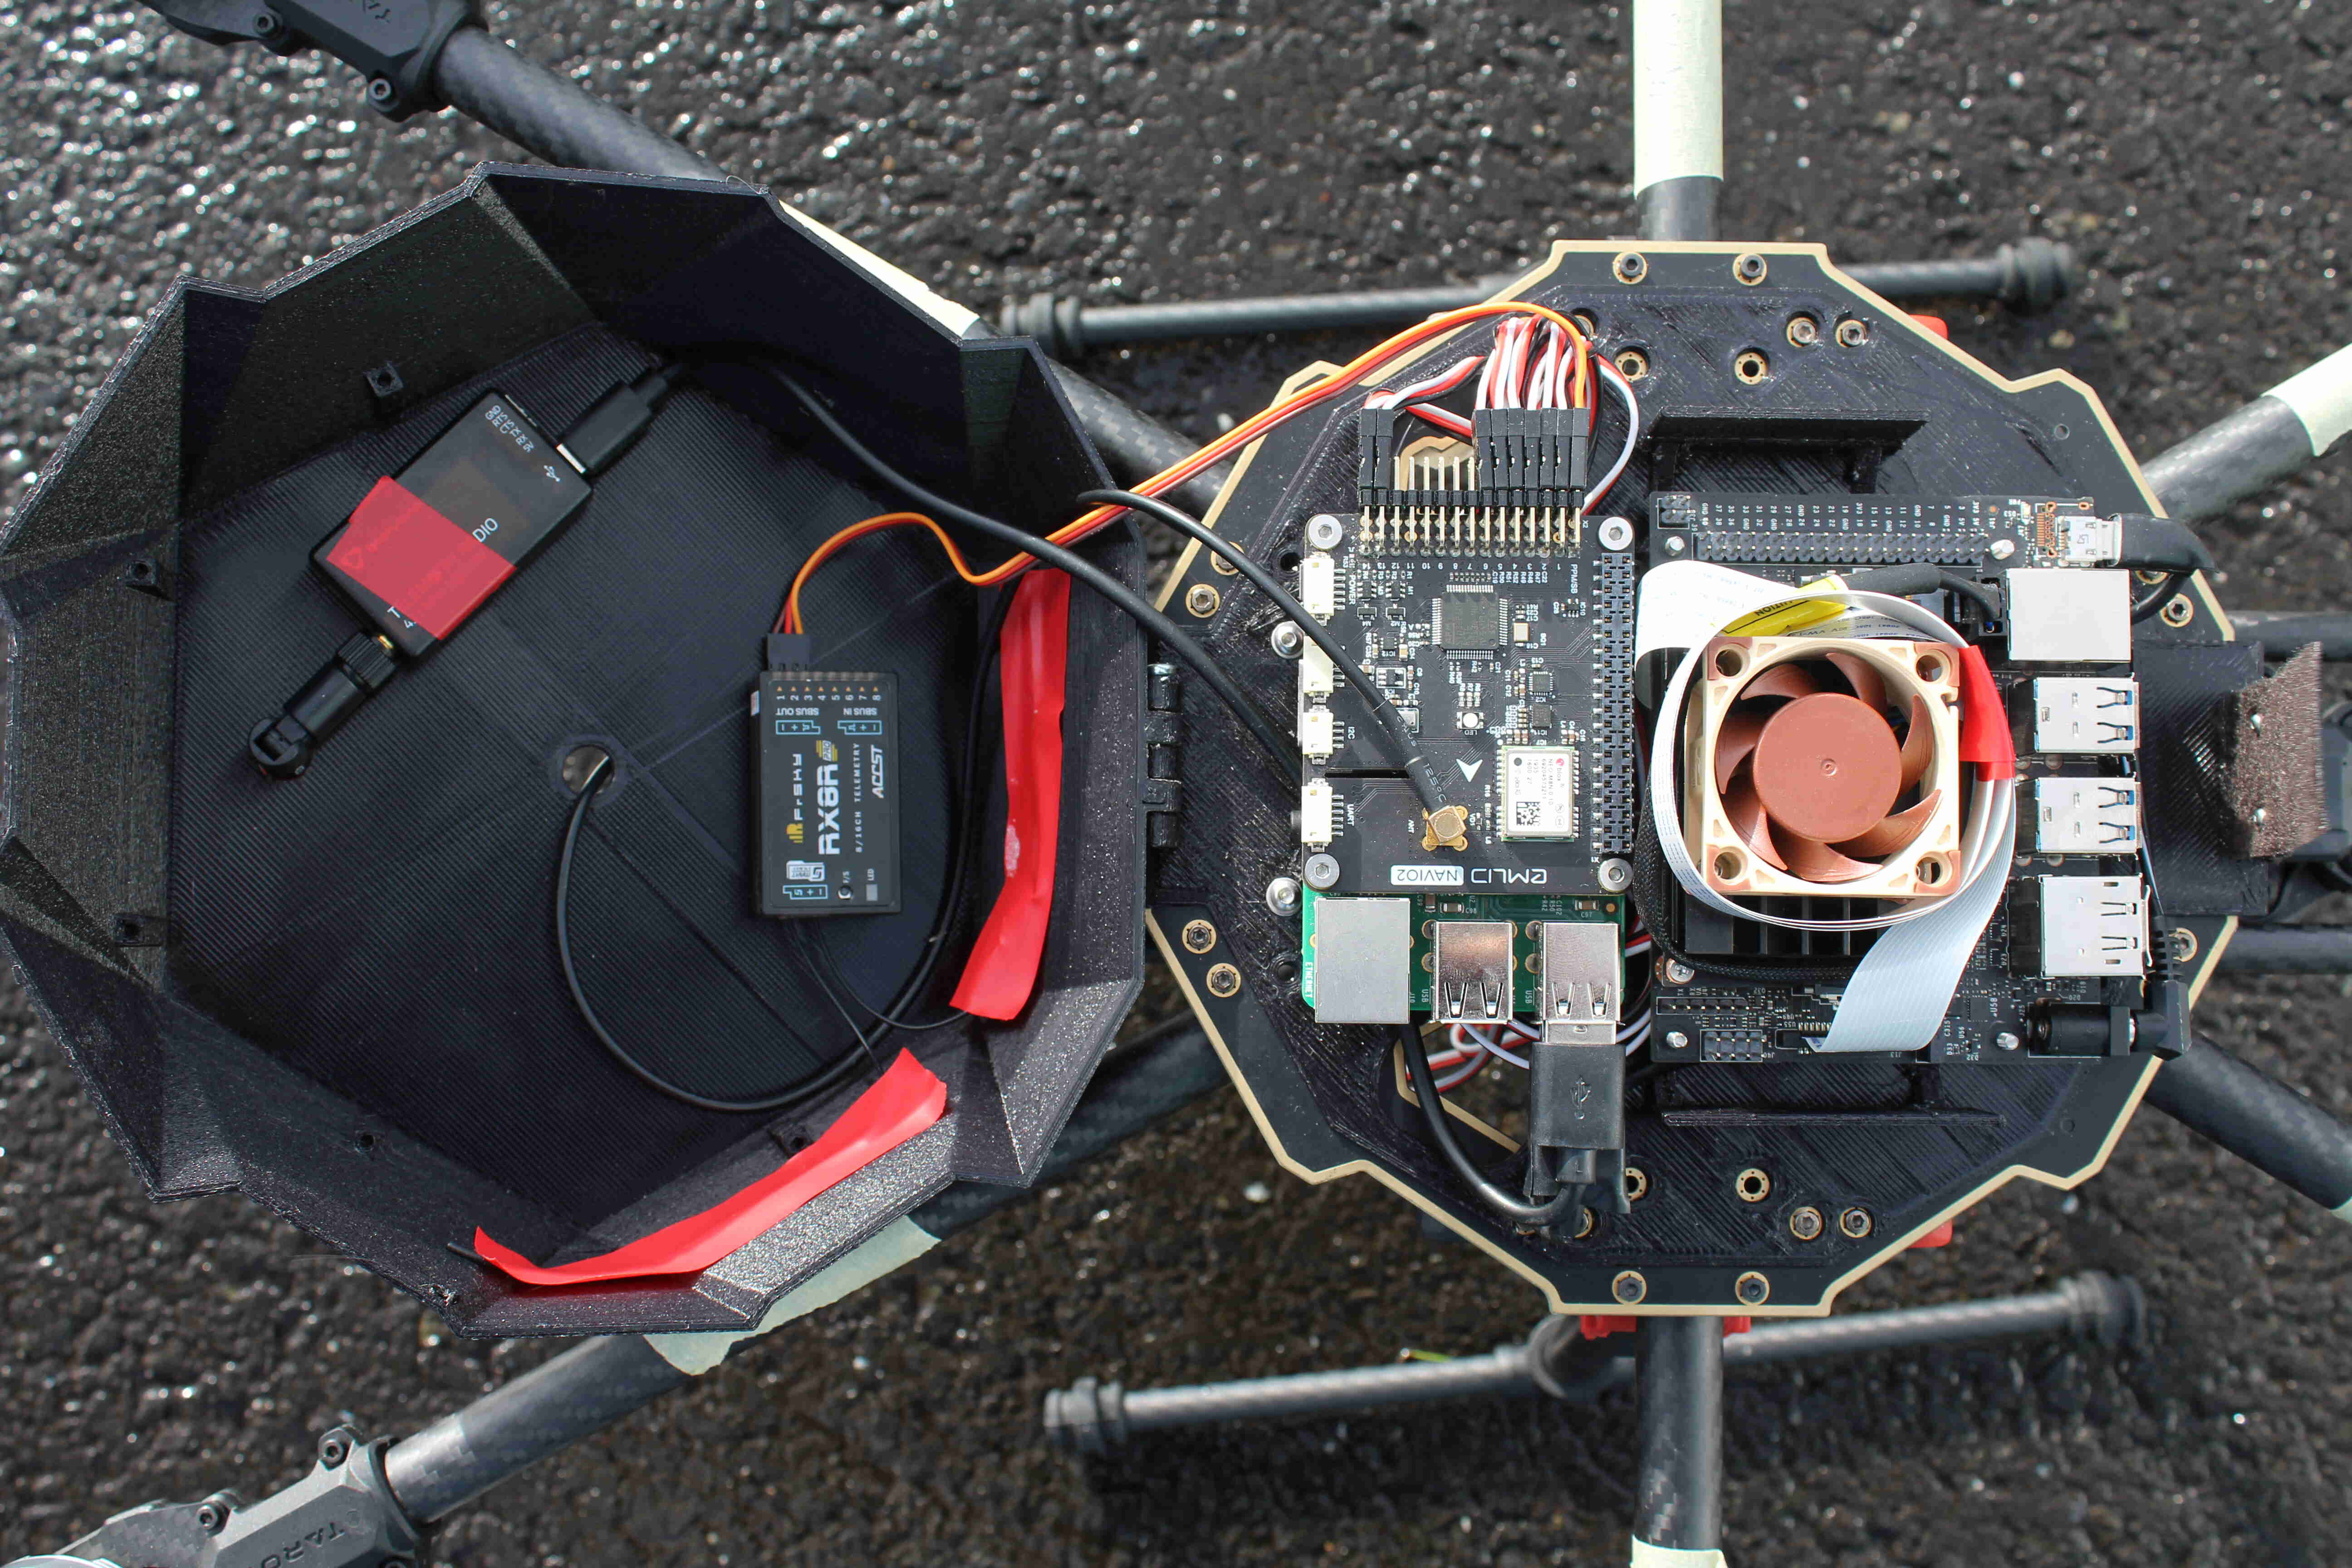
\includegraphics[width=0.6\textwidth]{jetson_electronics}\\
  \end{columns}
\end{frame}

\begin{frame}
  \frametitle{Test Hexacopters' Performance}
  \begin{columns}
    \column{0.5\textwidth}
    \begin{itemize}
      \item Stable (manual) flight performance
      \mypause
      \item \textasciitilde 20 min flying time
      \mypause
      \item Successful marker tracking
      \mypause
      \item Errors during approach
      \begin{itemize}
        \item Monocular pose estimation ambiguity
        \mypause
        \item GPS inaccuracy
      \end{itemize}
      \mypause
      \item No successful autonomous landing\\(but almost)
    \end{itemize}
    \column{0.5\textwidth}
    \centering
    {
    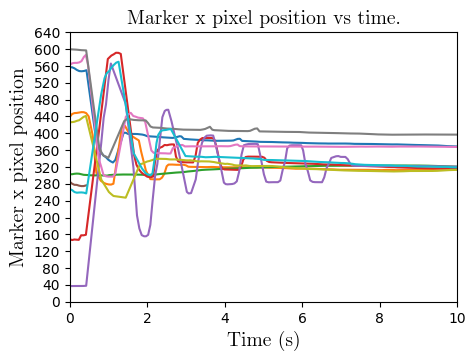
\includegraphics[width=0.6\textwidth]{coral_gimbal_performance_x_axis}\\
    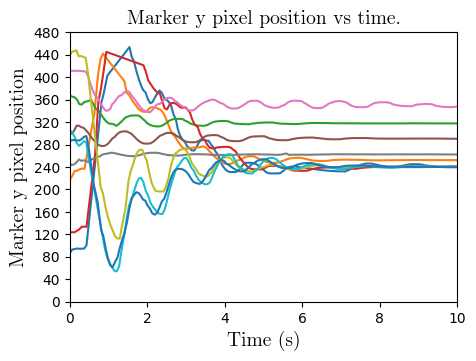
\includegraphics[width=0.6\textwidth]{coral_gimbal_performance_y_axis}\\
    }
  \end{columns}
\end{frame}

\begin{frame}
  \frametitle{Heavy Lift IR Drone}
  \begin{columns}
    \column{0.4\textwidth}
    \begin{itemize}
      \item Project with Christopher Hamilton (geologist, University of Arizona) and Baldur Björnsson
      \mypause
      \item 1.3 m span, 25 kg lift
      \mypause
      \item FLIR camera
      \mypause
      \item Surveyed lava field at Fagradalsfjall
      \mypause
      \item Featured \href{https://youtu.be/6SIgFPhhRPE?t=1208}{\color{blue}on BBC Click}
    \end{itemize}
    \column{0.5\textwidth}
    \centering
    \onslide
    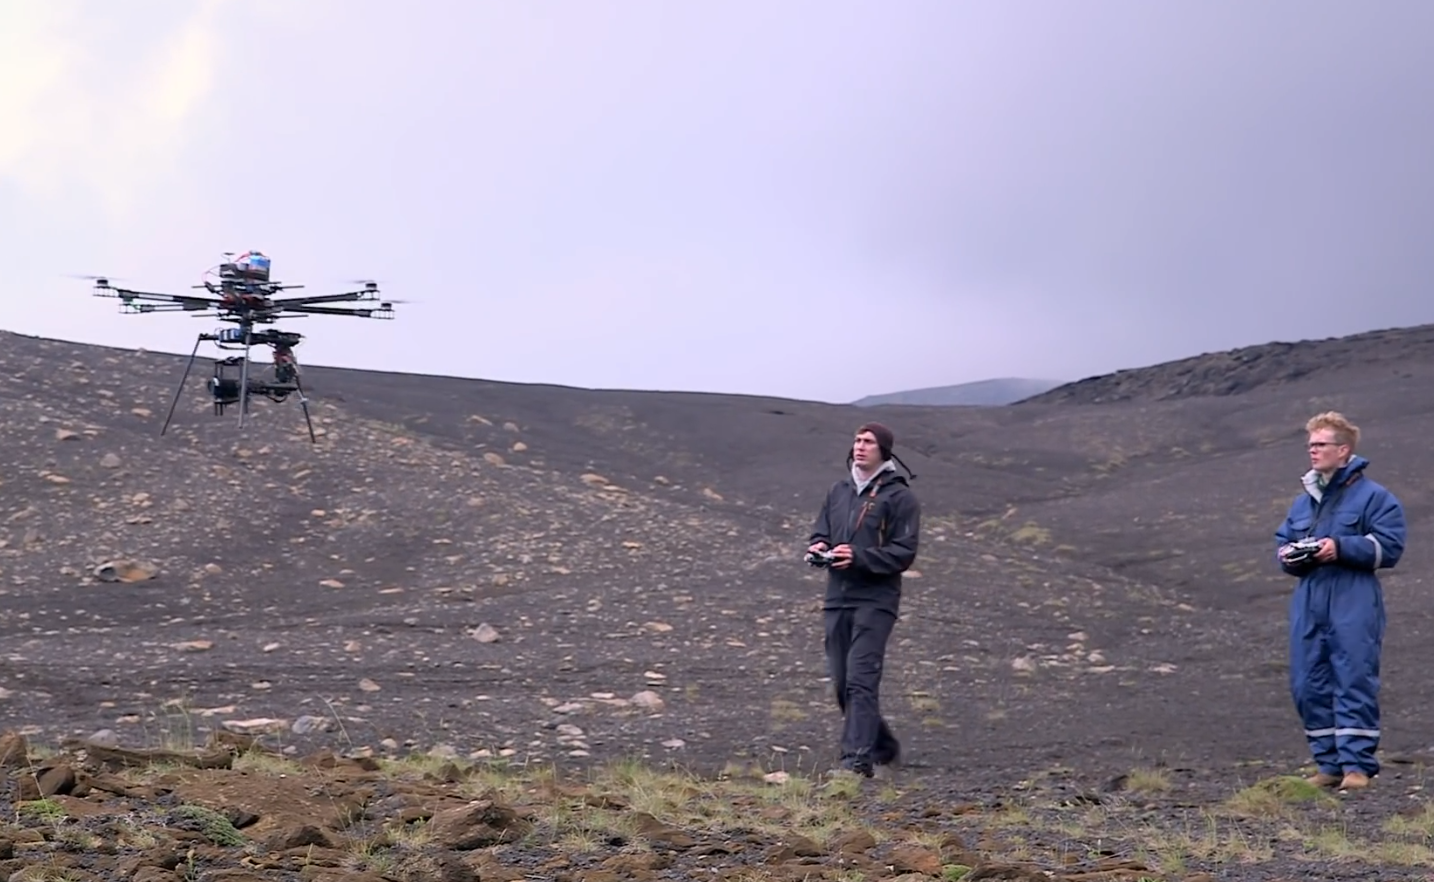
\includegraphics[width=0.7\textwidth]{ir_drone_in_flight}
    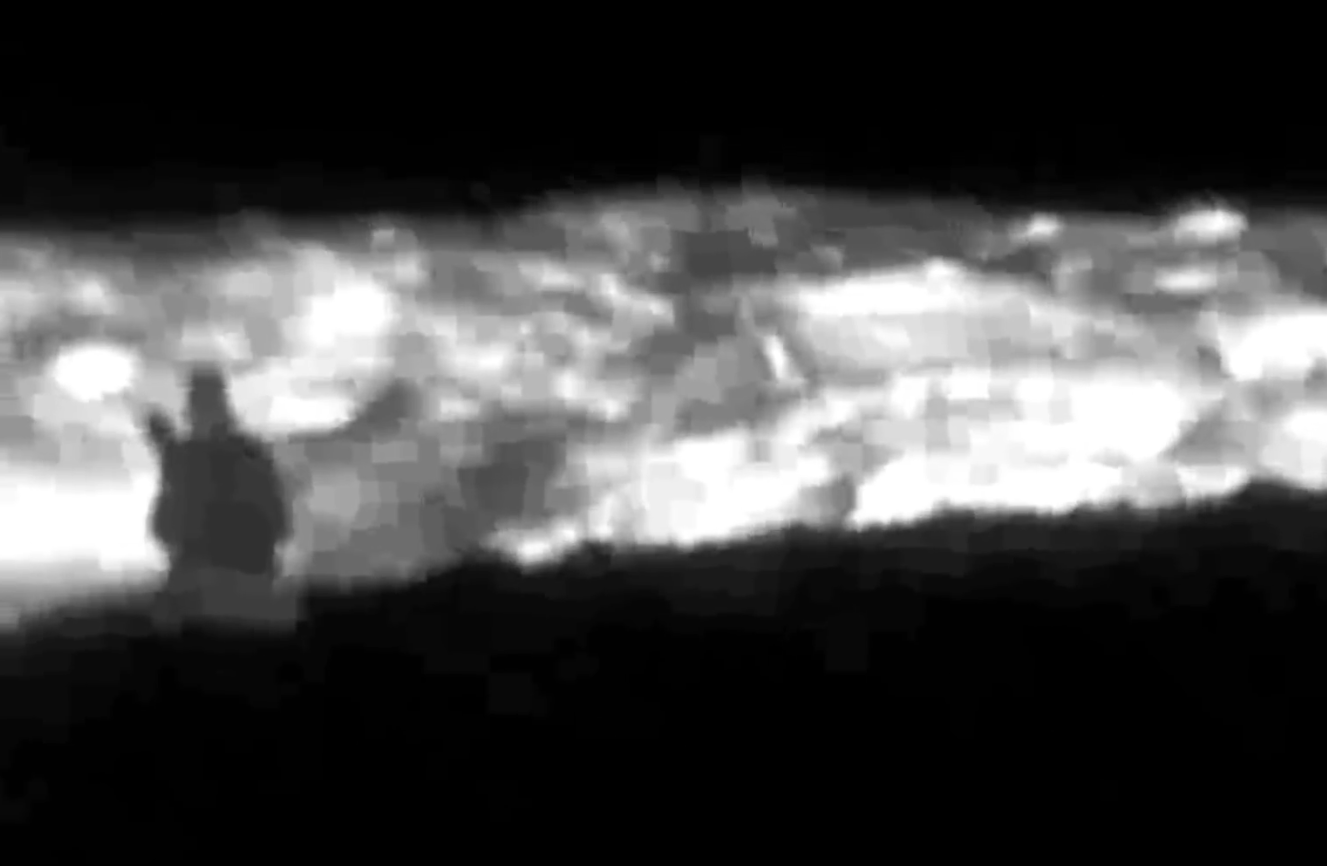
\includegraphics[width=0.7\textwidth]{ir_drone_ir_stillframe}
  \end{columns}
\end{frame}

\nologo
\begin{frame}
  \frametitle{Fiducial System Modifications}
  \begin{columns}

    \column{0.5\textwidth}
    Necessary properties:
    \begin{itemize}
      \item Mitigates orientation ambiguity
      \mypause
      \item Detectable at long- and short-range
      \mypause
      \item Runs on embedded hardware
    \end{itemize}
    \column{0.5\textwidth}
    \centering
    \onslide
    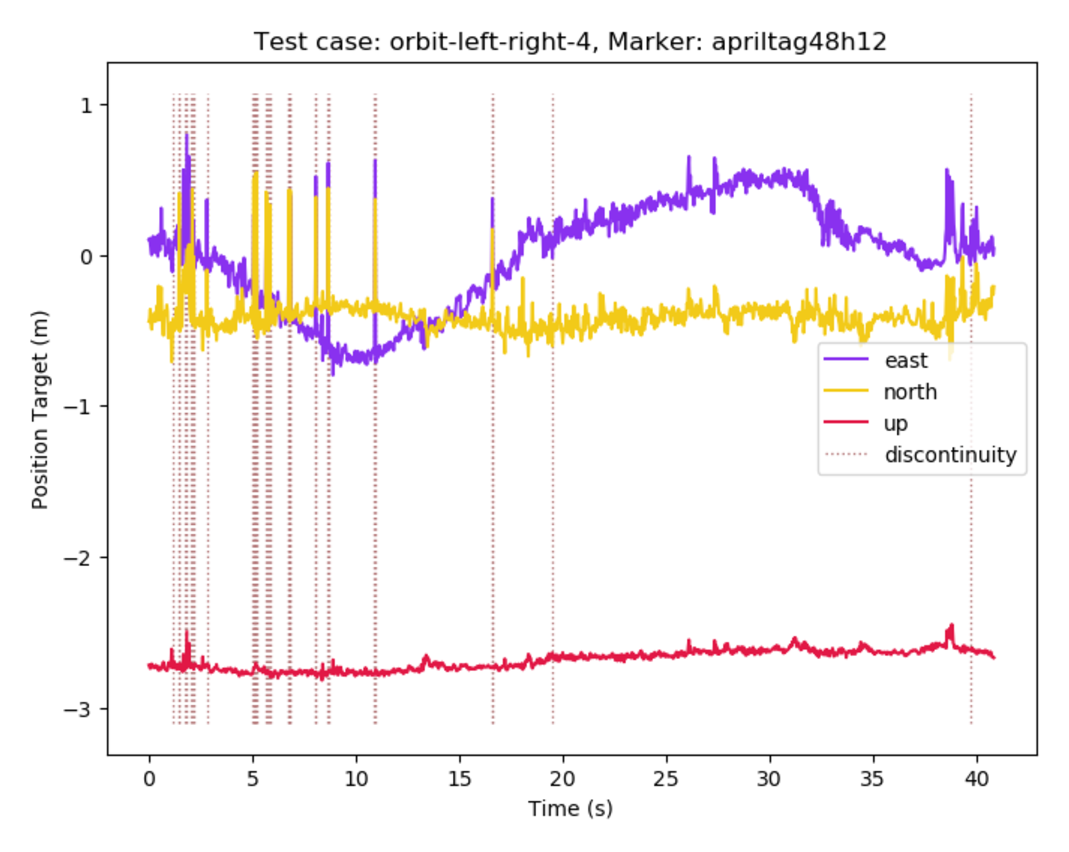
\includegraphics[width=0.9\textwidth]{orbit-left-right-4_apriltag48h12_position-target}
  \end{columns}
\end{frame}

\begin{frame}
  \frametitle{Orientation Ambiguity in WhyCode}
  \begin{columns}
    \column{0.5\textwidth}
    \begin{itemize}
      \item Semi-axes~\textrightarrow~2 possible orientations
      \mypause
      \item Better centered~\textrightarrow~correct
      \mypause
      \item Arclength of intersections with ID ``teeth''
    \end{itemize}
    \column{0.5\textwidth}
    \centering
    \onslide
    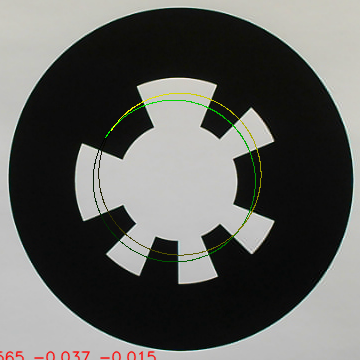
\includegraphics[width=0.9\textwidth]{whycode_orig_both_solutions_cropped}
  \end{columns}
\end{frame}

\begin{frame}
  \frametitle{Fiducial System Modifications: ``WhyCode Ellipse''}

  \begin{columns}
    \column{0.5\textwidth}
    Approach 1: Extra tooth sampling
    \begin{itemize}
      \mypause
      \item Sample ID with original method.
      \mypause
      \item Add: radial sampling on tooth edges.
      \mypause
      \item Choose solution based on tooth edge predictions.
    \end{itemize}
    \column{0.5\textwidth}
    \centering
    \onslide
    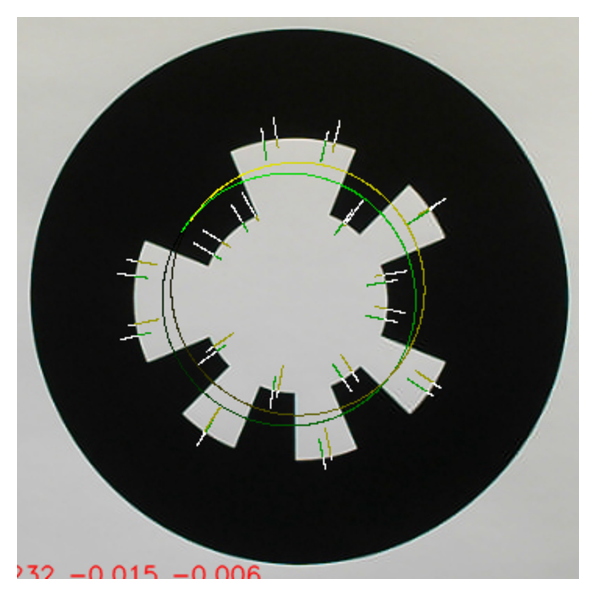
\includegraphics[width=0.9\textwidth]{whycode_ellipse_both_solutions_cropped}\\
  \end{columns}
\end{frame}

\begin{frame}
  \frametitle{Fiducial System Modifications: ``WhyCode Multi''}

  \begin{columns}
    \column{0.5\textwidth}
    Approach 2: Coplanar marker arrangements
    \begin{itemize}
      \mypause
      \item Ignore individual marker orientations
      \mypause
      \item Calculate normal vector to the plane connecting the markers.
      \mypause
      \item Extract pitch and roll from the normal vector.
      \mypause
      \item Extract yaw from the marker IDs.
      \mypause
      \item Takes advantage of WhyCode's efficiency.
    \end{itemize}
    \column{0.5\textwidth}
    \centering
    \onslide
    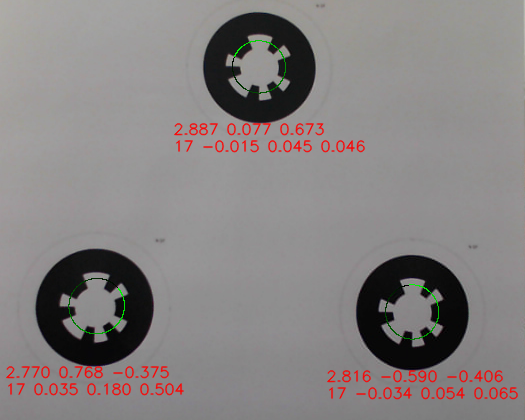
\includegraphics[width=0.9\textwidth]{cropped_whycode_3_8_jiri_example}
  \end{columns}
\end{frame}

\yeslogo
\begin{frame}
  \frametitle{Fiducial System Modifications: April Tag}
  April Tag: less orientation ambiguity, but less computationally efficient.\\
  \centering
  \vspace{1cm}
  \begin{tabular}{m{0.6\textwidth}m{0.15\textwidth}}
%    Tag 36h11: original, most common. Eclipses camera's field of view when viewed from too close. & 
\includegraphics[width=\linewidth]{tag_36h11_borderless}\\
    April Tag 48h12: more sophisticated, ``recursive.'' & 
\includegraphics[width=\linewidth]{tag48_12_00000}\\ & \\ & \\
    April Tag Custom 24h10: ``recursive,'' smaller definition & 
\includegraphics[width=\linewidth]{tag24_10_00000}
  \end{tabular}
\end{frame}

\nologo
\begin{frame}
  \frametitle{Performance Analysis: Discontinuity Rates}
  \begin{columns}
    \column{0.5\textwidth}
      \centering
      \begin{itemize}
        \item Orientation ambiguity~\textrightarrow~discontinuities.
        \item Discontinuity rate $\overline{r_d}$ is the number of discontinuities per detection.
        \item Lower is better.
      \end{itemize}
    \column{0.5\textwidth}
      \centering
      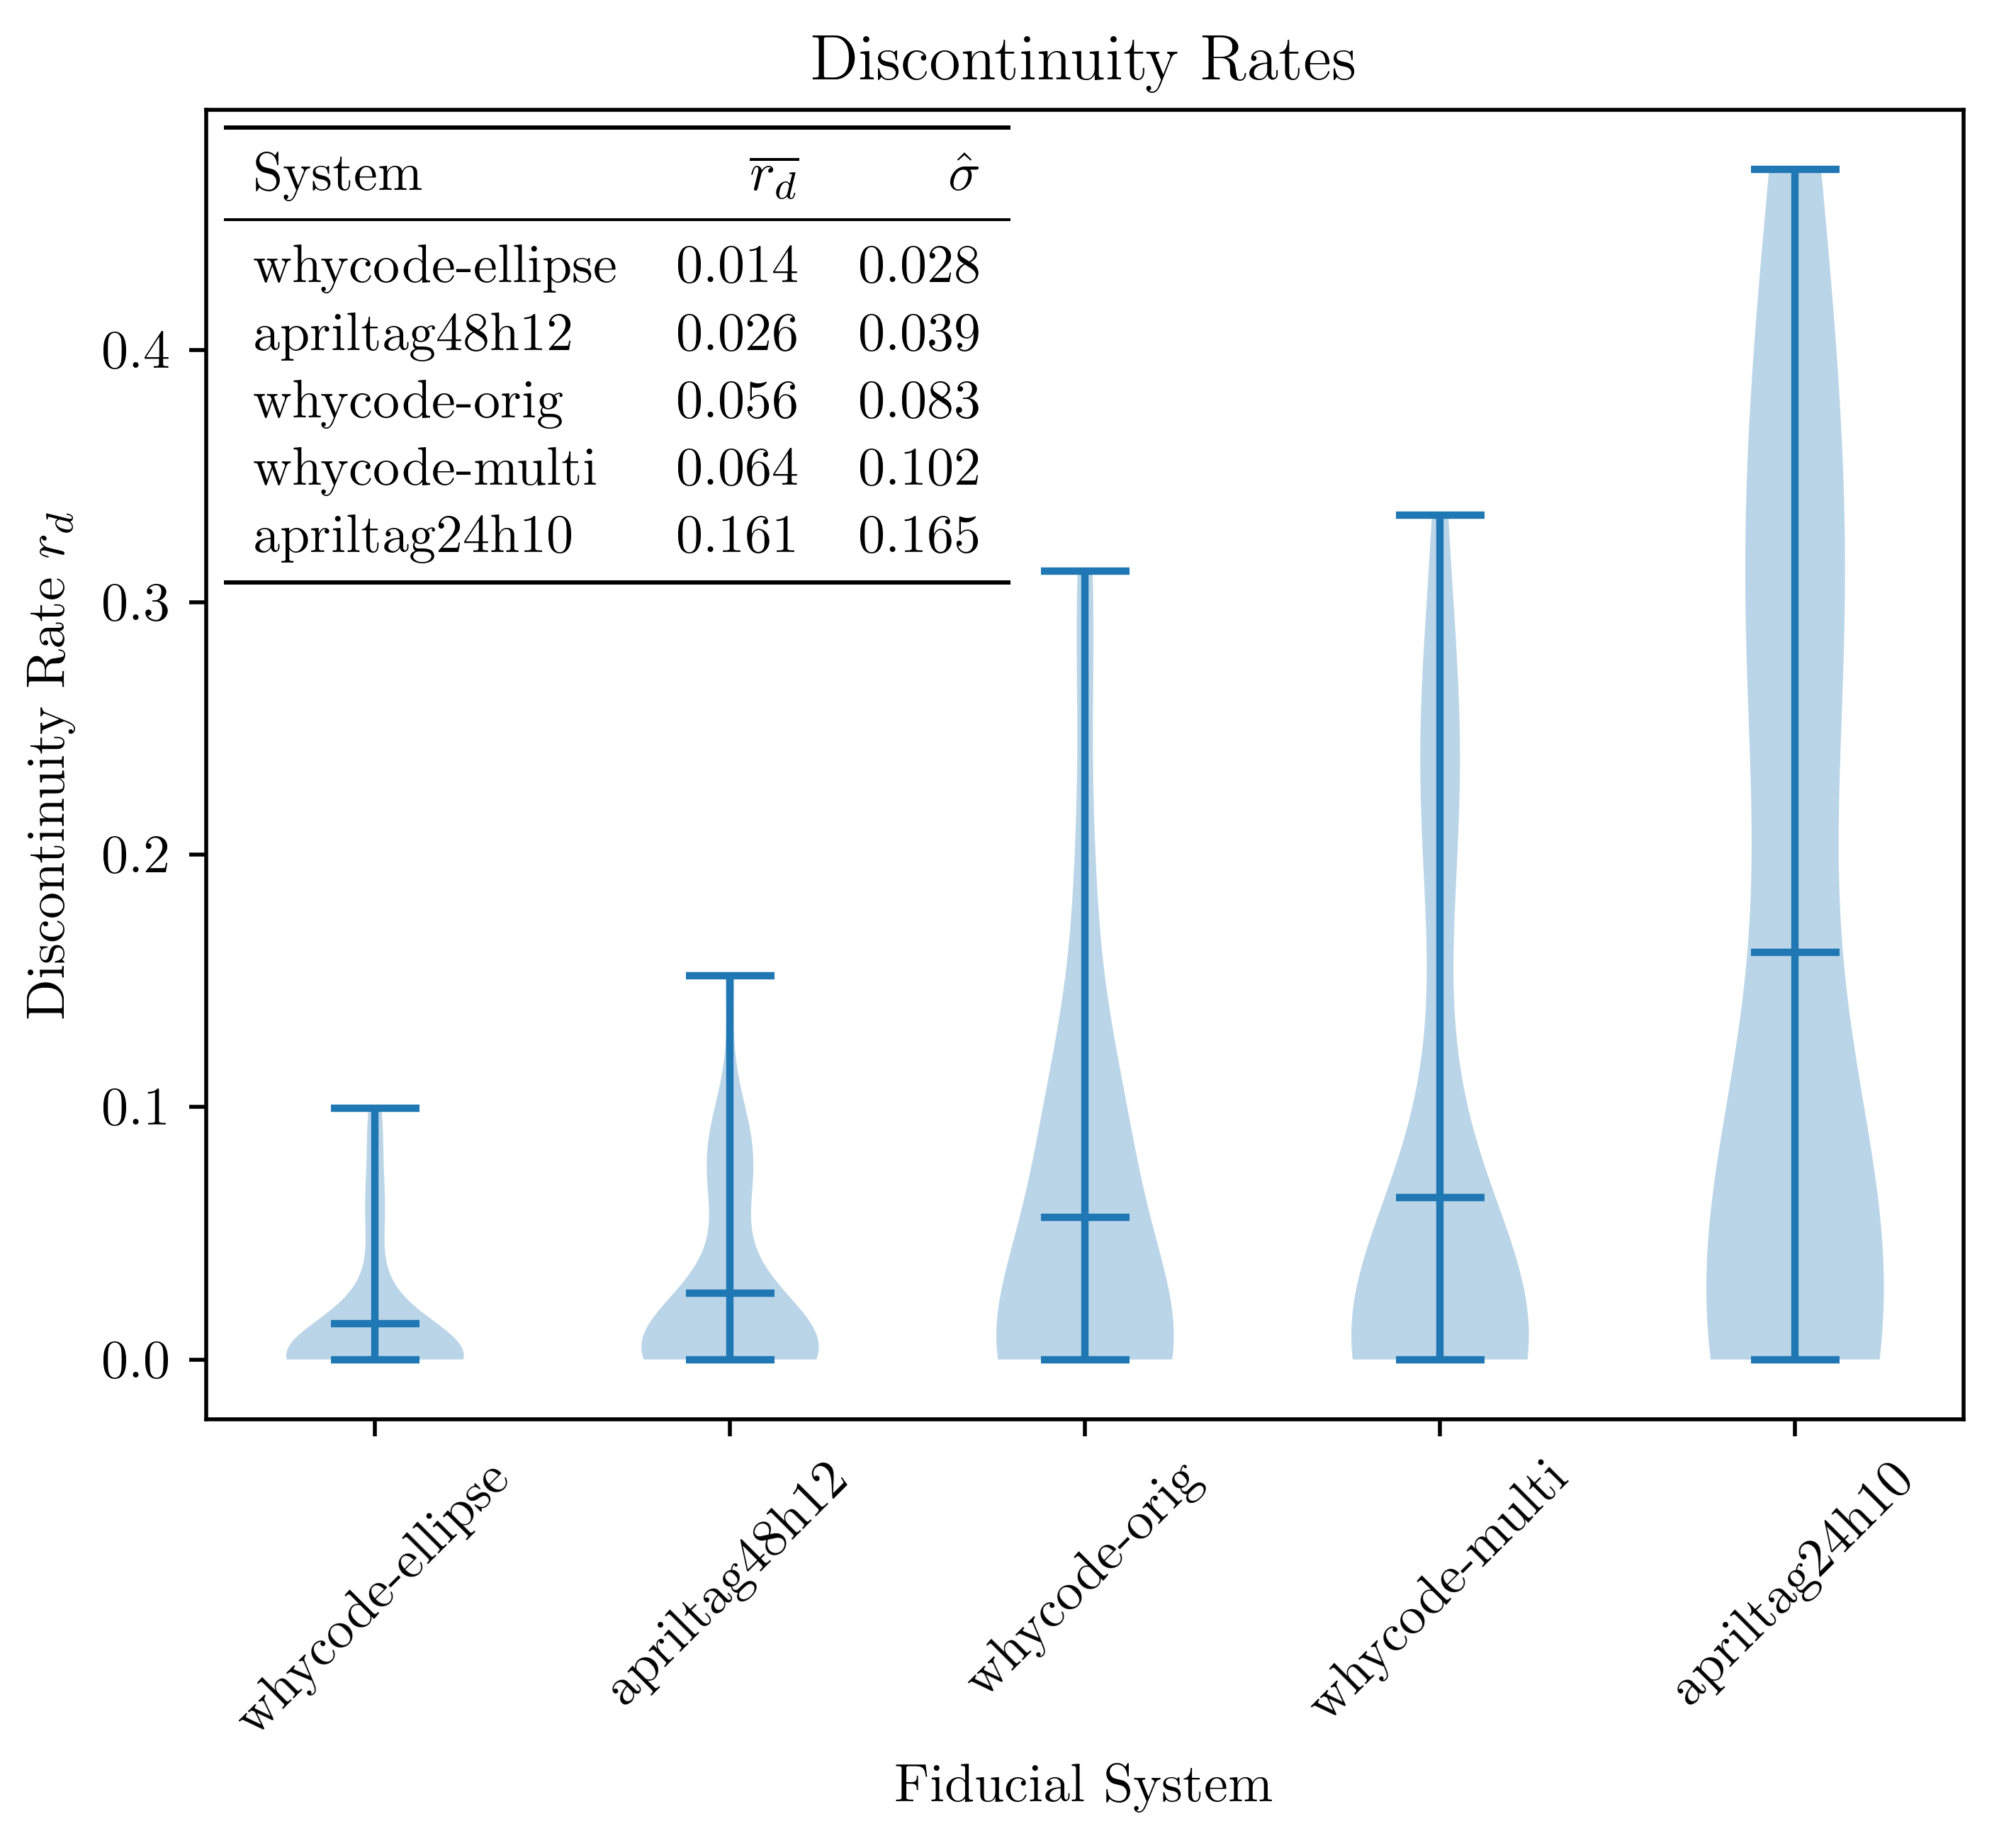
\includegraphics[width=\textwidth]{violin_plot_five_member}
  \end{columns}
\end{frame}

\begin{frame}
  \frametitle{Performance Analysis: Detection Rates}
  \begin{columns}
    \column{0.5\textwidth}
      \centering
      \begin{itemize}
        \item Detection rate $\overline{F}$ is the number of detections per second.
        \item Tested on Raspberry Pi 4.
        \item Higher is better.
      \end{itemize}
    \column{0.5\textwidth}
      \centering
      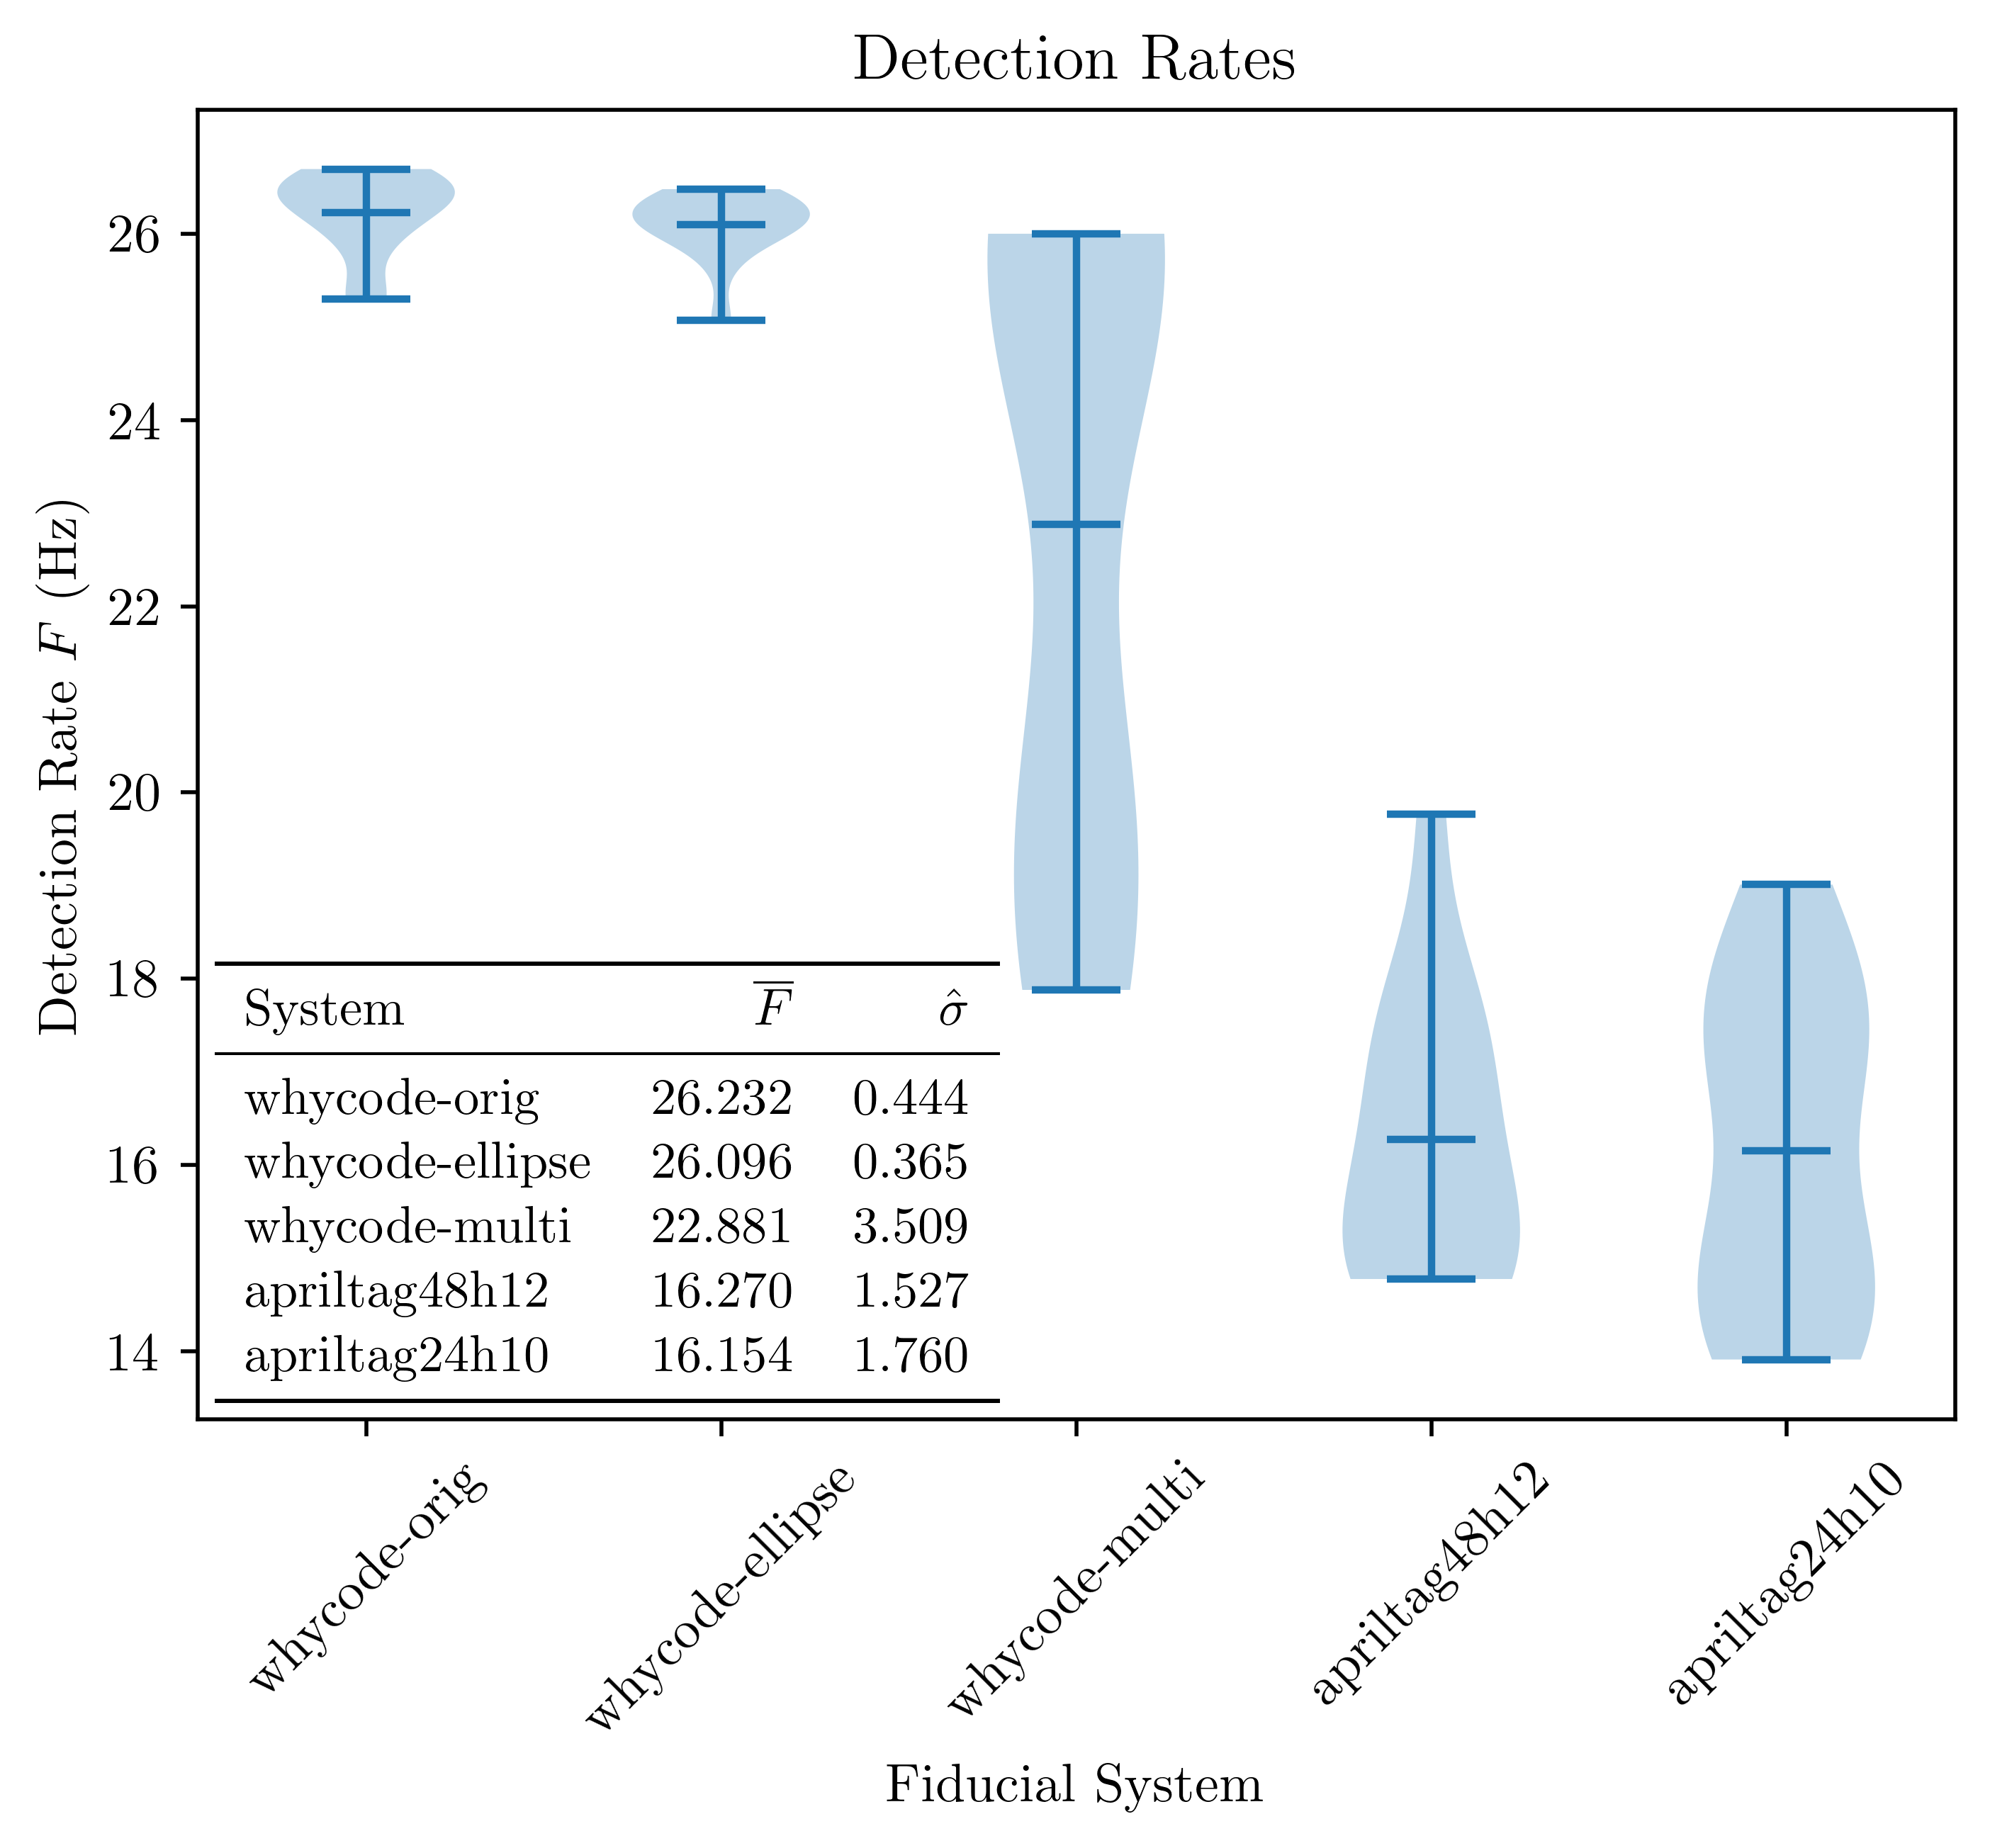
\includegraphics[width=\textwidth]{violin_plot_speed_five_member}
  \end{columns}
\end{frame}

\begin{frame}
  \frametitle{Autonomous Landing Proof of Concept}
  \begin{columns}
    \column{0.5\textwidth}
      \begin{itemize}
        \item Indoor experiments with DJI Spark
        \mypause
        \begin{itemize}
          \item Reduces logistical considerations:\\transportation, weather
          \mypause
          \item Stable out-of-the-box autonomous flight
          \mypause
          \item Doesn't require GPS (uses other sensors)
        \end{itemize}
        \mypause
        \item Requires DJI Mobile SDK, Custom Android App, and \textbf{lots} of workarounds.
        \mypause
        \item Video frames are offloaded (via WiFi) to Raspberry Pi 4 for processing
        \mypause
        \item Limiting factor: pre-transmission image compression on tablet (6-7 Hz)
      \end{itemize}
    \column{0.5\textwidth}
    \centering
    \onslide
    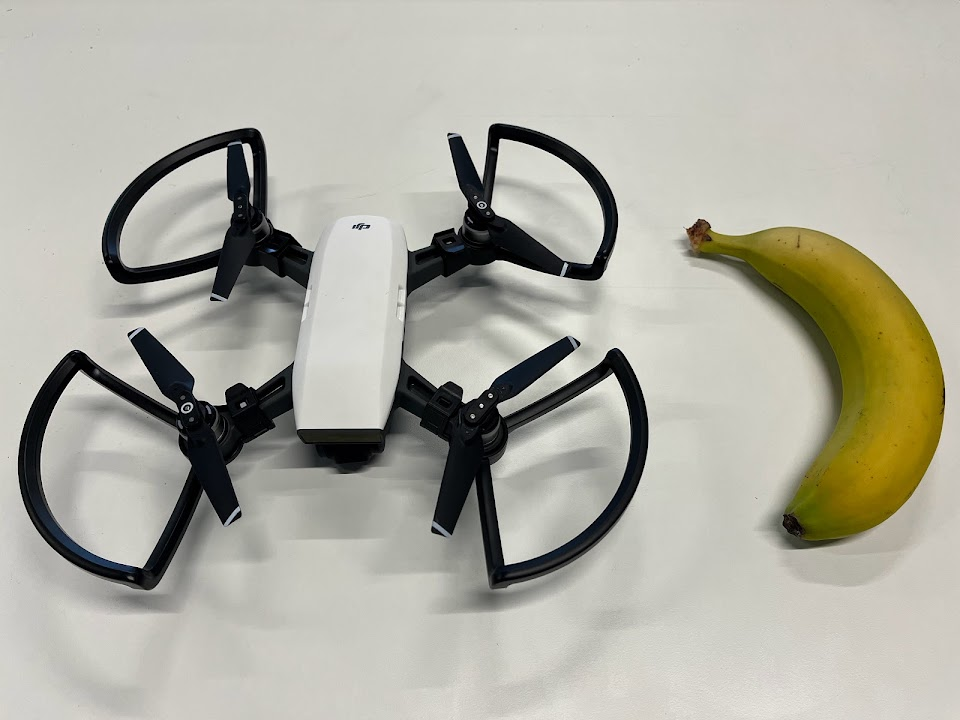
\includegraphics[width=\textwidth]{dji_spark}\\(Banana for scale.)
  \end{columns}
\end{frame}

\begin{frame}
  \frametitle{Autonomous Landing Proof of Concept: System Architecture}
  
\includegraphics[width=\textwidth]{spark_architecture.drawio}
\end{frame}

\begin{frame}
  \frametitle{Demo with worst-performing April Tag 24h10!}
  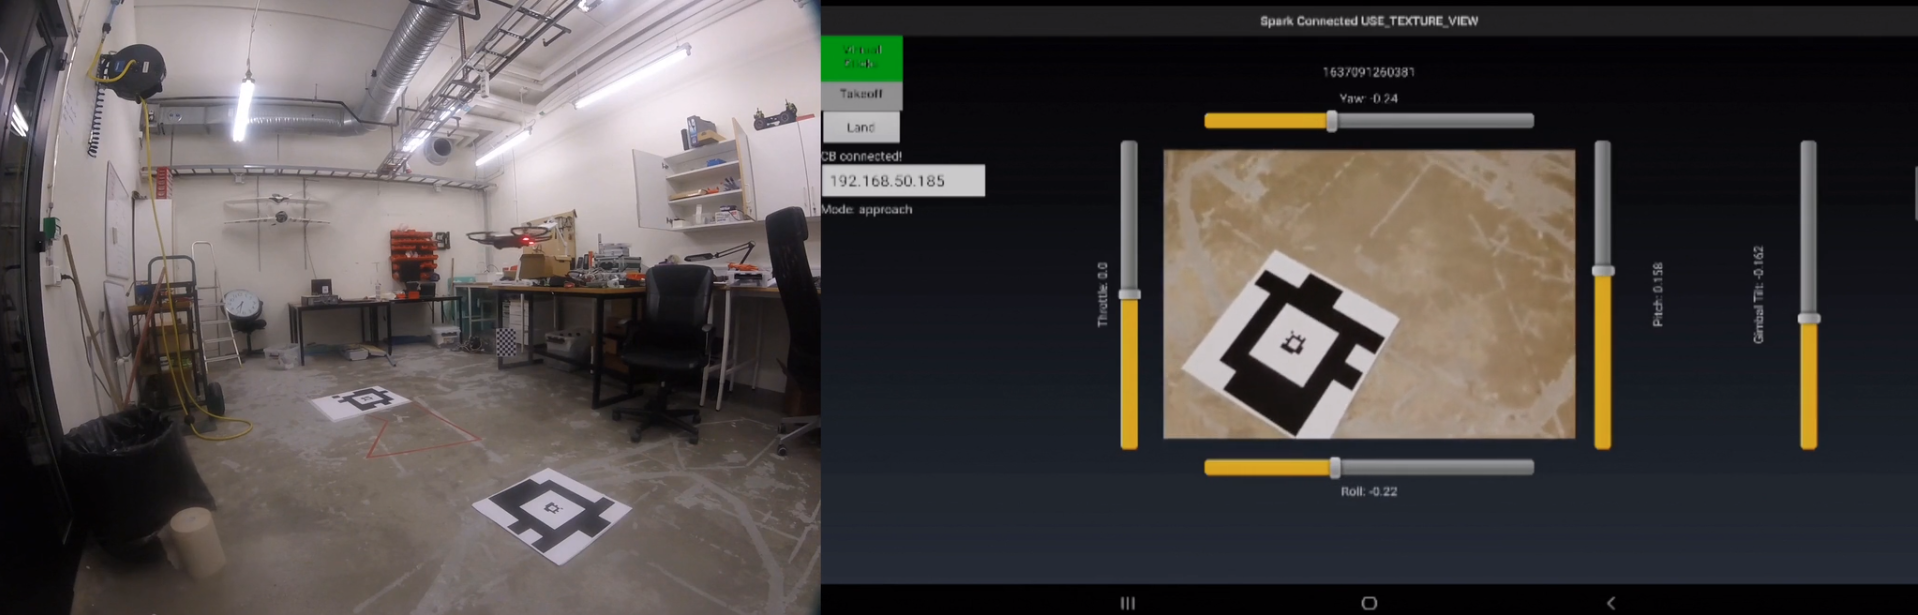
\includegraphics[width=\textwidth]{demo_screenshot}
%  \href{https://vimeo.com/664863992}{\color{blue}Click to watch on Vimeo}
\end{frame}

\yeslogo
\begin{frame}
  \frametitle{Publications}
  \begin{itemize}
    \item Submitted: Evaluation of April Tag and WhyCode Fiducial Systems for Autonomous Precision Drone Landing with a Gimbal-Mounted Camera
    \item In Progress: results from autonomous landing proof of concept
  \end{itemize}
\end{frame}

\section{Research Plan}

\begin{frame}
  \frametitle{Overview: Unstructured Autonomous Landing}
  \begin{itemize}
    \item Focus on terrain analysis
    \begin{itemize}
      \mypause
      \item Topographical analysis%\mypause: (smoothness, slant, flatness, size of flat regions)
      \mypause
      \item Semantic segmentation%\mypause: terrain type classification%\mypause: label terrain according to
      \begin{itemize}
        \item terrain type classification: (snow, ice, water, grass, rock, etc.)
        \mypause
        \item classify according to predicted safety: (safe, questionable, unsafe, etc.)
      \end{itemize}
    \end{itemize}
    \mypause
    \item Focus on real time performance
    \begin{itemize}
      \mypause
      \item Minimize computational requirements
      \mypause
      \item Target specific hardware platforms
    \end{itemize}
    \mypause
    \item Overall structure:
    \begin{itemize}
      \item Input: sensor data
      \item Process (quickly): ??
      \item Output: safe landing sites (e.g. heat map)\mypause~\textrightarrow~flight control commands
    \end{itemize}
%    \item Approach:
%    \begin{itemize}
%      \item Input: sensor data (RGBD, LIDAR, RADAR)
%      \mypause
%      \item Topographical analysis: signal processing or deep learning methods
%      \item Semantic segmentation: deep learning methods% CNN, U-net or Residual U-net% for semantic segmentation
%      \mypause
%      \item Pre-processing wrappers:
%      \begin{itemize}
%        \item Rectification/calibration of images/point clouds
%        \mypause
%        \item Downsampling of input resolution
%%        \mypause
%%        \item Topological analysis
%      \end{itemize}
%      \mypause
%      \item Potential post-processing wrappers
%      \begin{itemize}
%        \item Safe landing site tracking
%        \mypause
%        \item Translation to flight commands
%      \end{itemize}
%    \end{itemize}
  \end{itemize}
\end{frame}

\begin{frame}
  \frametitle{Data Set Generation}
  \begin{columns}
    \column{0.5\textwidth}
      AirSim: realistic simulator
      \begin{itemize}
        \item Automatic generation of large data sets
        \mypause
        \item Synthetic sensor data (LIDAR, RGBD cameras)
        \mypause
        \item Tag with IMU data
        \mypause
        \begin{itemize}
          \item LIDAR~\textrightarrow~RADAR
        \end{itemize}
        \mypause
        \item Specify realistic sensor parameters
        \mypause
        \item Segmentation masks for high-level label generation
        \mypause
        \item Labeling method can be slow, hand-tuned
      \end{itemize}
    \column{0.5\textwidth}
      \onslide
      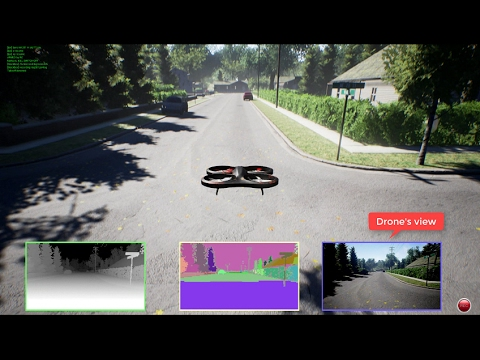
\includegraphics[width=0.9\textwidth]{airsim}

      \href{https://mspoweruser.com/microsoft-launches-aerial-informatics-and-robotics-platform-to-help-developers-build-autonomous-systems/}{\color{blue}Image source}
    \centering
  \end{columns}
\end{frame}

\begin{frame}
  \frametitle{Terrain Classifier Creation}
  \begin{columns}
    \column{0.5\textwidth}
      \begin{itemize}
        \item Test several methods
        \mypause
        \begin{itemize}
          \item Conventional signal/image processing%(gradient analysis, edge detection)
          \mypause
          \item Deep learning methods% (CNN, U-net, Residual U-net)
          \mypause
          \item Combination
        \end{itemize}
        \mypause
        \item Pre-processing wrappers:
        \begin{itemize}
          \item Rectification/calibration
          \mypause
          \item Downsampling/resizing
        \end{itemize}
        \mypause
        \item Performance comparison
        \begin{itemize}
          \item Reduce false positives
          \mypause
        \end{itemize}
      \end{itemize}
    \column{0.5\textwidth}
    \centering
    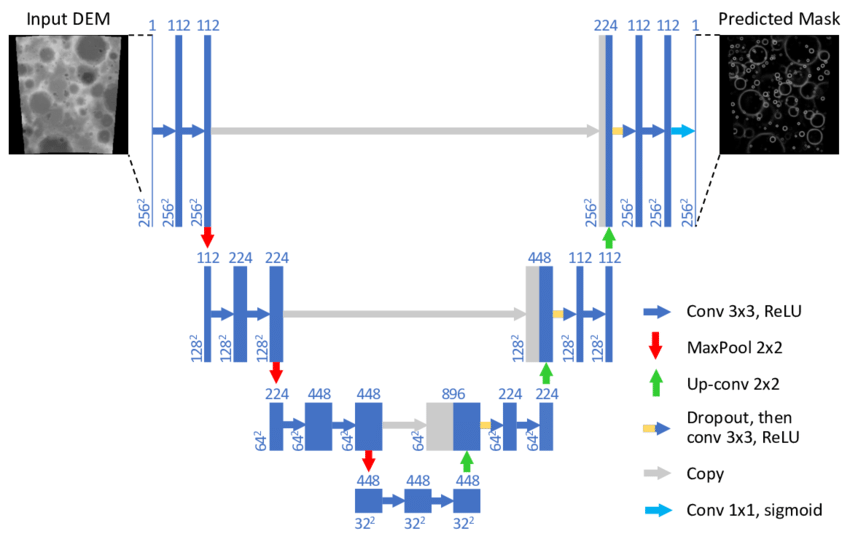
\includegraphics[width=\textwidth]{Convolutional-neural-network-CNN-architecture-based-on-UNET-Ronneberger-et-al}\\
    \href{https://www.researchgate.net/figure/Convolutional-neural-network-CNN-architecture-based-on-UNET-Ronneberger-et-al_fig2_323597886}{Image source}
  \end{columns}
\end{frame}

\begin{frame}
  \frametitle{Testing in Simulation}
  \begin{columns}
    \column{0.9\textwidth}
    \begin{itemize}
      \item Post-processing wrappers:
      \begin{itemize}
        \item Safe region tracking
        \mypause
        \item Translation to flight commands
      \end{itemize}
      \mypause
      \item Integration with ArduPilot/PX4 SITL
      \mypause
      \item Simulated autonomous missions in AirSim
      \mypause
      \item Qualitative analysis:
      \begin{itemize}
        \item Does the drone land at all?
        \mypause
        \item Does the safe region tracking work?
        \mypause
        \item Does the autopilot software accept the commands?
      \end{itemize}
    \end{itemize}
    \column{0.1\textwidth}
    \centering
  \end{columns}
\end{frame}

\section{Simulation is not enough!}

%\nologo
%\begin{frame}
%  \frametitle{Testing in the Real World}
%  \begin{columns}
%    \column{0.6\textwidth}
%    \begin{itemize}
%      \item<1-> Offline
%      \begin{itemize}
%        \item<1-> Accuracy on real world data
%      \end{itemize}
%      \mypause
%      \item<2-> Lab scenarios
%      \begin{itemize}
%        \item<3-> Runtime framerate on embedded hardware
%        \item<3-> Power requirements on embedded hardware
%      \end{itemize}
%      \mypause
%      \item<4-> Real world landing scenarios
%    \end{itemize}
%    \column{0.4\textwidth}
%    \centering
%    \visible<2->{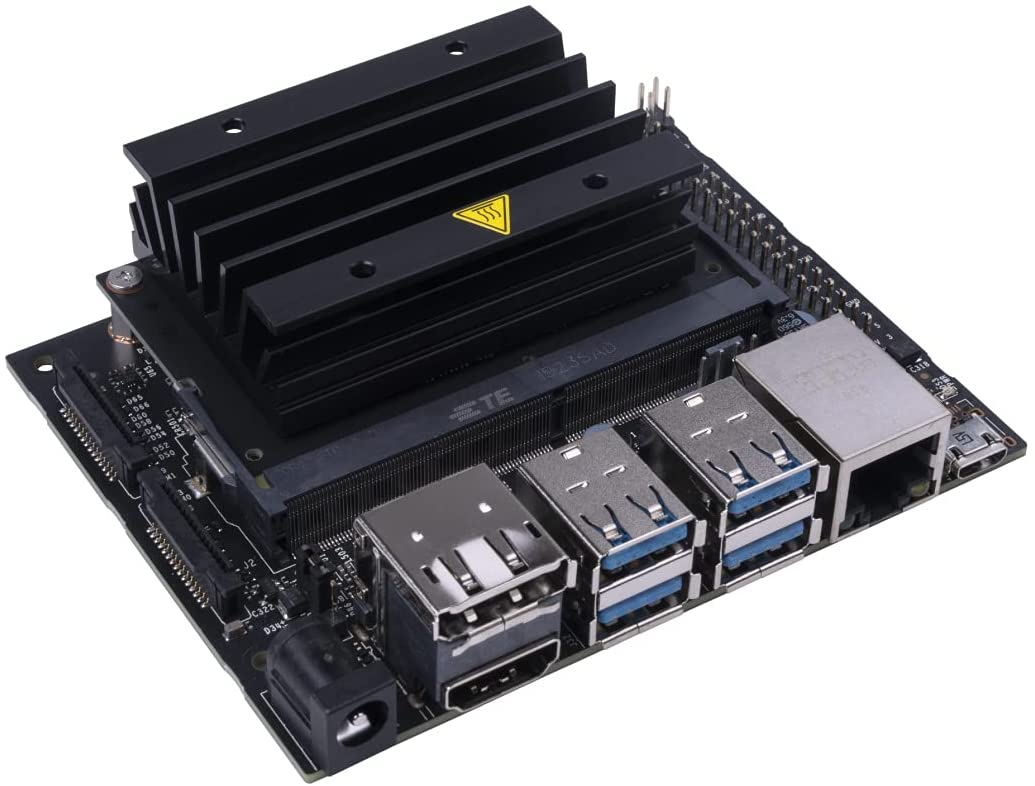
\includegraphics[width=0.75\textwidth]{jetson_nano}\\}
%    \visible<2->{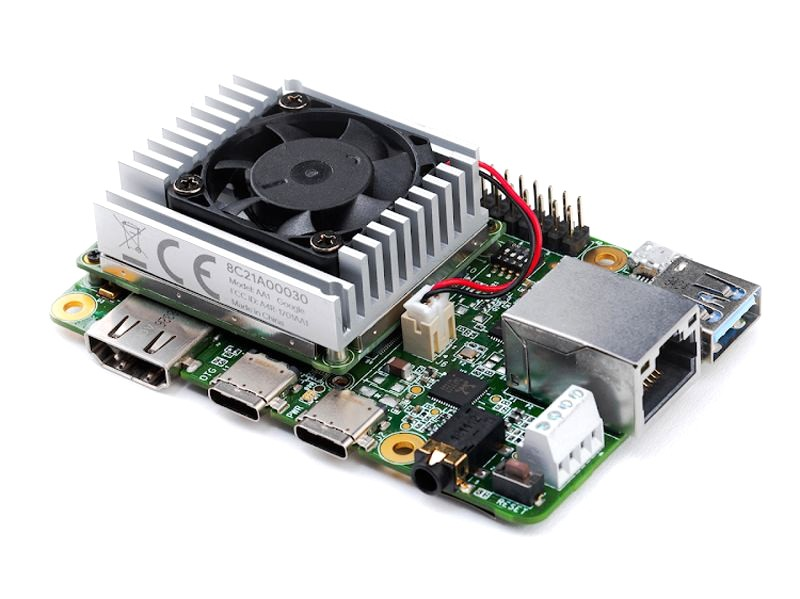
\includegraphics[width=0.75\textwidth]{google_coral}}
%    \mypause
%  \end{columns}
%\end{frame}

\nologo
\begin{frame}
  \frametitle{Testing in the Real World}
  \begin{columns}
    \begin{column}{0.6\textwidth}
      \begin{itemize}
        \item<1-> Offline
        \begin{itemize}
          \item<1-> Accuracy on real world data
        \end{itemize}
%        \mypause
        \item<2-> Lab scenarios
        \begin{itemize}
          \item<2-> Runtime framerate on embedded hardware
          \item<2-> Power requirements on embedded hardware
        \end{itemize}
        \mypause
        \item<3-> Real world landing scenarios
      \end{itemize}
    \end{column}
    \visible<1->
    {
      \begin{column}{0.4\textwidth}
      \centering
        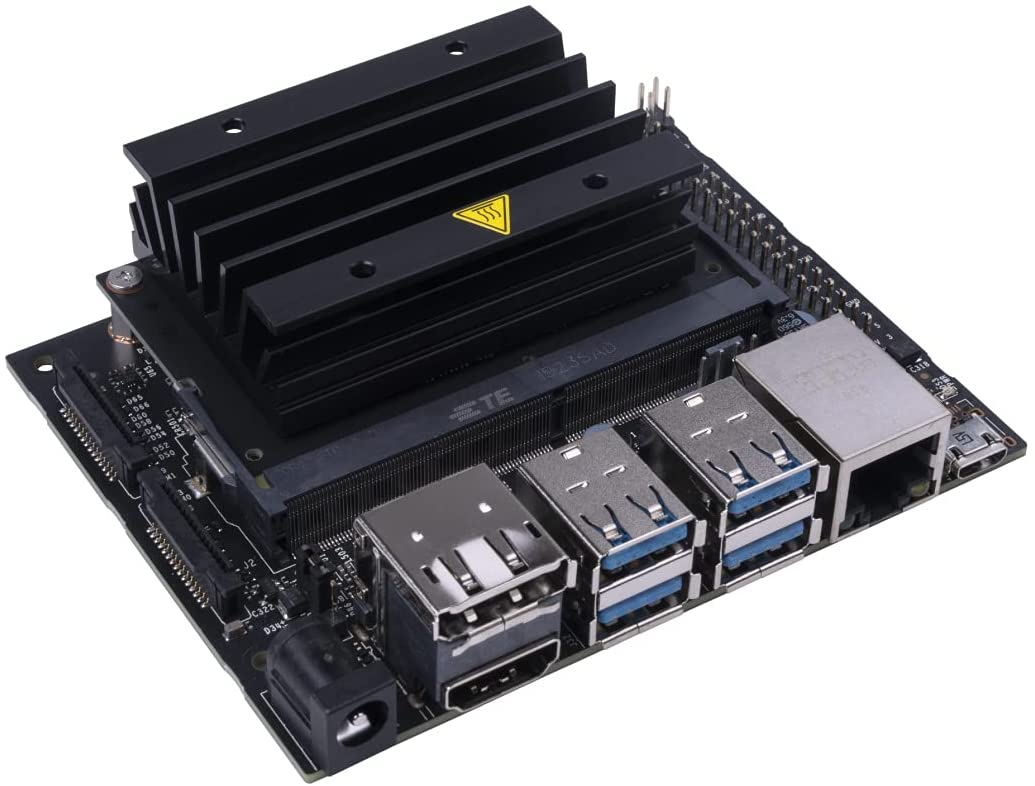
\includegraphics[width=0.75\textwidth]{jetson_nano}\\
        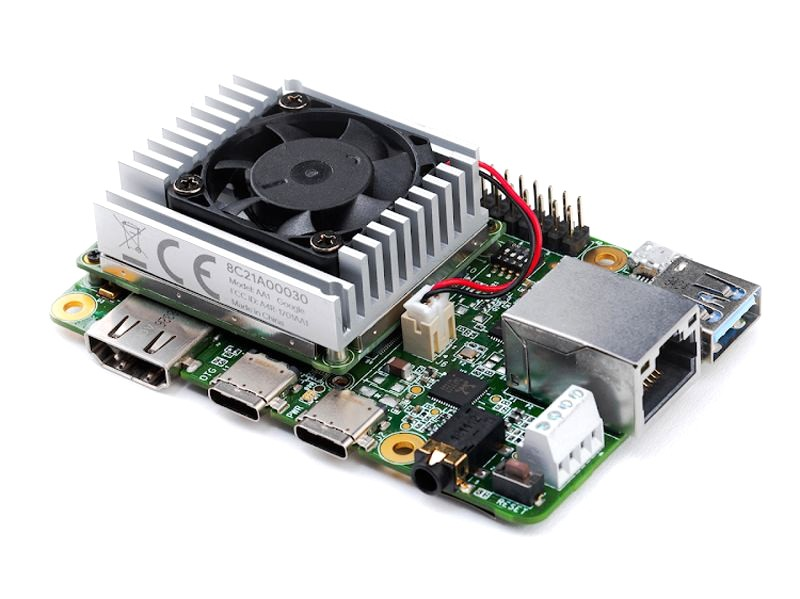
\includegraphics[width=0.75\textwidth]{google_coral}
      \end{column}
    }
    \mypause
  \end{columns}
\end{frame}

\yeslogo
\begin{frame}
  \frametitle{Drone Upgrades}
  \begin{columns}
    \column{0.6\textwidth}
      \begin{itemize}
        \item New flight controller: Pixhawk Cube Orange
        \mypause
        \item Here3
        \mypause
        \item Supplement GPS
        \mypause
        \begin{itemize}
          \item Optical Flow
          \item LIDAR rangefinder
        \end{itemize}
        \mypause
        \item Protective sensor cases, gimbal mounts
        \mypause
        \begin{itemize}
          \item Intel RealSense D435 RGBD camera
          \item Intel RealSense D455 RGBD camera (IMU)
          \item Intel RealSense L515 LIDAR (IMU)
          \item Texas Instruments IWR6843 60 GHz RADAR
        \end{itemize}
      \end{itemize}
    \column{0.4\textwidth}
    \centering
    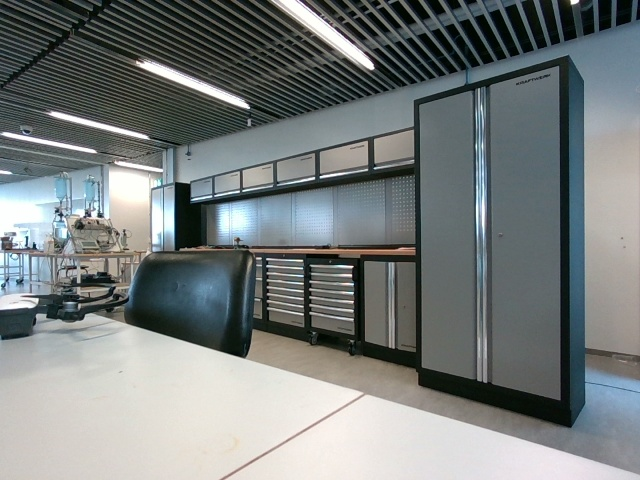
\includegraphics[width=0.75\textwidth]{rgb_image}\\
    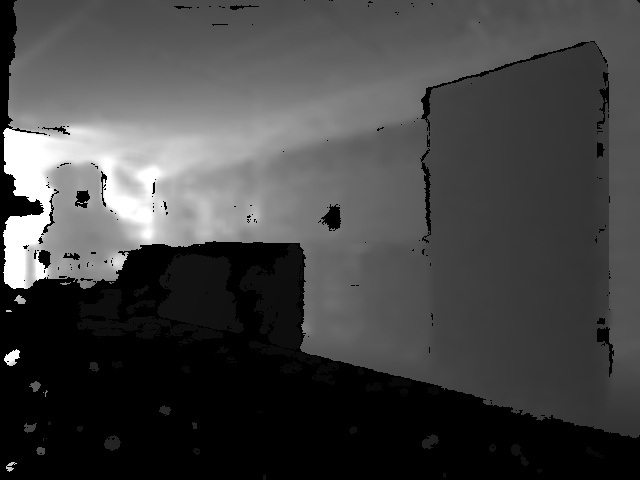
\includegraphics[width=0.75\textwidth]{depth_image}
  \end{columns}
\end{frame}

\begin{frame}
  \frametitle{Main Risks}
  \begin{itemize}
    \item The synthetic data does not accurately represent the real world!
    \mypause
    \begin{itemize}
      \item Show results in simulation.
      \mypause
      \item Use real world data\mypause~\textrightarrow~no segmentation masks.
    \end{itemize}
    \mypause
    \item The embedded hardware is too slow!
    \mypause
    \begin{itemize}
      \item Reduce computational needs\mypause~\textrightarrow~prune network, decrease input data size\mypause
      \item Use non-embedded hardware\mypause~\textrightarrow~generate reliable flight commands on real world data
    \end{itemize}
  \end{itemize}
\end{frame}

\begin{frame}
  \frametitle{Summary}
  \begin{columns}
    \column{0.5\textwidth}
      \begin{itemize}
        \item Goal: autonomous drone landing
        \mypause
        \item Past work: landing via fiducial markers at \textit{known} landing pads
        \begin{itemize}
          \item Contribution: gimbal-mounted camera setup, new marker variants
        \end{itemize}
        \mypause
        \item Research plan: unstructured landing
        \begin{itemize}
          \mypause
          \item Sensors: RGBD, LIDAR/RADAR
          \mypause
          \item Topographical/semantic terrain analysis
          \mypause
          \item Synthetic data
          \mypause
          \item Testing in simulation
          \mypause
          \item Real world tests: power/framerate
          \mypause
          \item Real world tests: landing with a physical drone
          \mypause
        \end{itemize}
        \item Thank you! Are there any questions?
      \end{itemize}

    \column{0.5\textwidth}
      \centering

      \onslide
      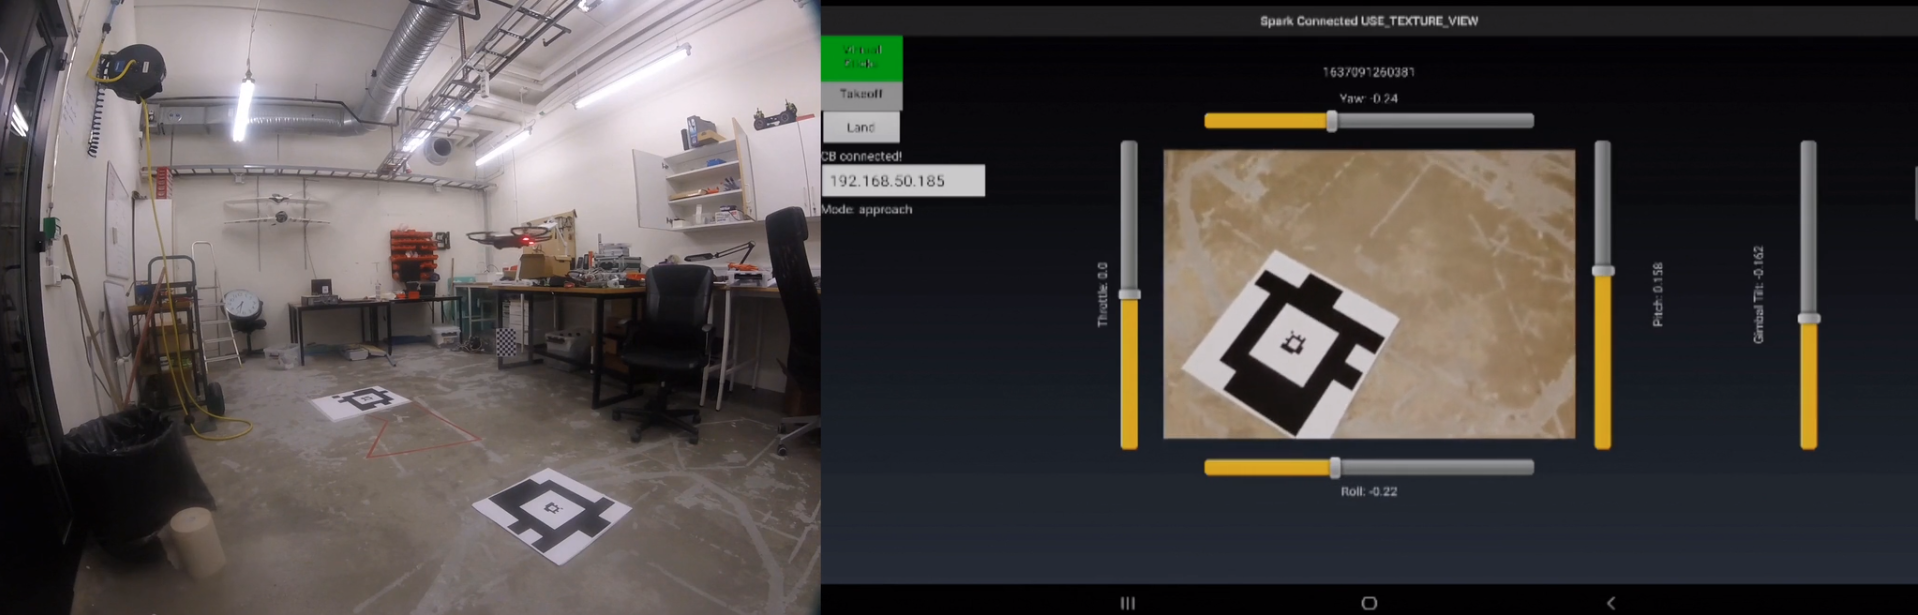
\includegraphics[width=\textwidth]{demo_screenshot}\\\href{https://vimeo.com/664863992}{\color{blue}Click to watch on Vimeo}\vspace{1cm}

      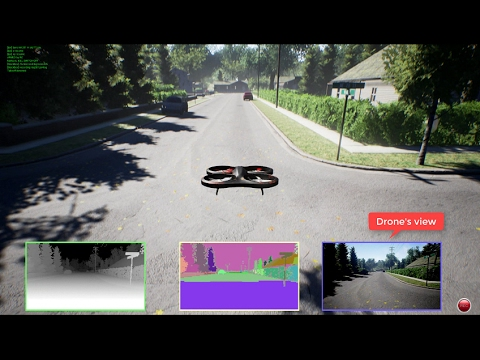
\includegraphics[width=0.5\textwidth]{airsim}
  \end{columns}
\end{frame}

\begin{frame}[allowframebreaks]
  \frametitle{References}
  \printbibliography{}
\end{frame}

\end{document}